
%%%%%%%%%%%%%%%%%%%%%%%%%%%%%%%%%%%%%%%%%%%%%%%
\setcounter{table}{0}
\setcounter{figure}{0}
\setcounter{section}{0}
\pagenumbering{gobble}
% APPENDIX 
\pagenumbering{arabic}
\renewcommand\thefigure{OA-\arabic{figure}}
\renewcommand\thetable{OA-\arabic{table}}
\renewcommand*{\thepage}{OA - \arabic{page}}
\renewcommand\thesection{Appendix \Alph{section}.}
\renewcommand\thesubsection{\Alph{section}.\arabic{subsection}}

\newgeometry{margin=1in}
\begin{center}
	\Large ONLINE APPENDIX: The controlled choice design and private paternalism in pawnshop borrowing \\[0.5em]
	%\Large{Appendix $-$ For Online Publication} \\[1em]
	\large \author{Craig McIntosh \and Isaac Meza \and Joyce Sadka \and Enrique Seira \and Francis J.\ DiTraglia}
\end{center}


\begin{appendix}

    
%\section{ Treatment Explanation Materials and Pictures}
\section{Additional materials} 
%\vspace{.2in}
\begin{figure}[!h]
     \caption{Behavior of borrowers who lost their pawn.}
    \begin{center}
    \begin{subfigure}{0.35\textwidth}
        \caption{Elapsed days to first payment}
        \centering
        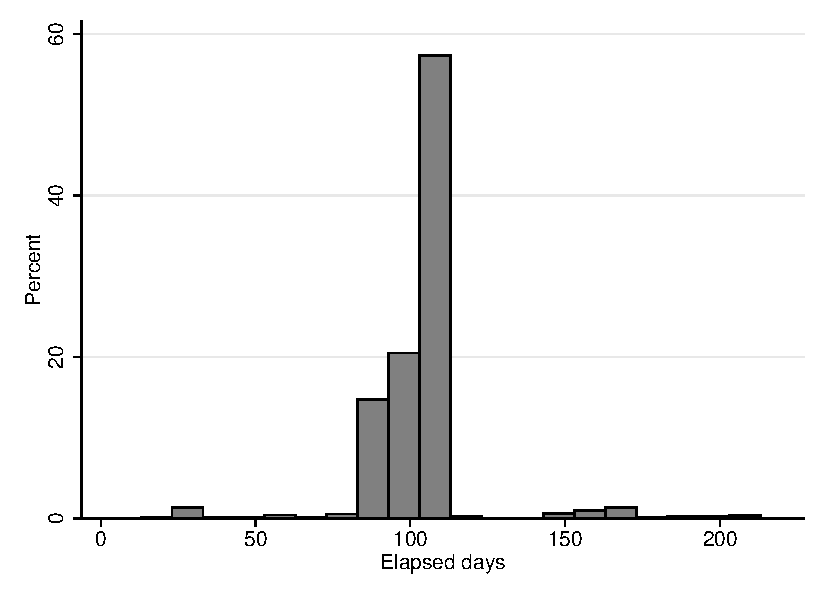
\includegraphics[width=\textwidth]{Figuras/hist_firstdays_default.pdf}
    \end{subfigure}
    \begin{subfigure}{0.35\textwidth}
        \caption{Elapsed days to last payment}
        \centering
        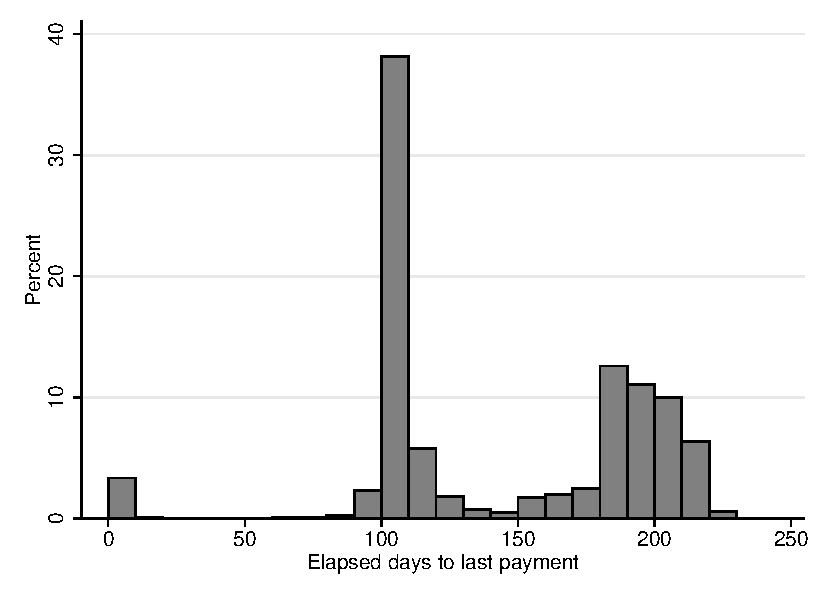
\includegraphics[width=\textwidth]{Figuras/hist_days_default.pdf}
    \end{subfigure}
        \begin{subfigure}{0.35\textwidth}
        \caption{Payments as \% of loan}
        \centering
        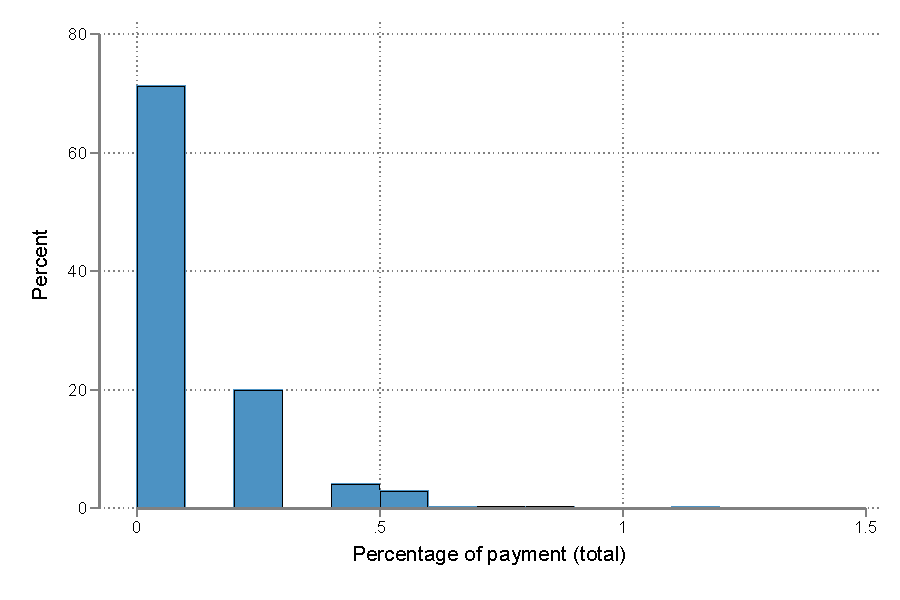
\includegraphics[width=\textwidth]{Figuras/hist_percpay_default.pdf}
    \end{subfigure}
    \begin{subfigure}{0.35\textwidth}
        \caption{Number of payments}
        \centering
        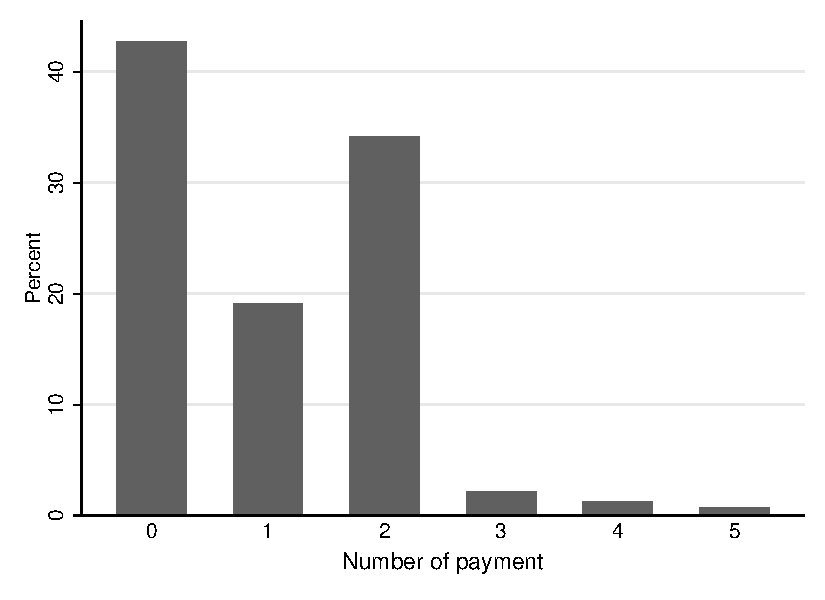
\includegraphics[width=\textwidth]{Figuras/hist_numpay_default.pdf}
    \end{subfigure}
    \end{center}
        \footnotesize{This figure provides more details on the behavior of clients who were assigned to the control group and did not recover their pawn. Panel (a) shows a histogram of days elapsed from the pawn to the first payment, while panel (b) displays a histogram of days elapsed until the last payment. Some borrowers make payments after day 105, the end of the grace period: if they pay all interest owed, they can ``restart'' the loan. This amounts to starting a new loan with the same conditions and same pawn. Panel (c) shows a histogram of the fraction of the loan paid, while panel (d) presents a barplot of the number of times that borrowers went to the branch to make payments.}
        \label{proxy_naive}
      %\textit{Do file: }  \texttt{hist\_den\_default.do}
\end{figure}

\begin{figure}[H]
    \caption{Determinants of choice.}
    \begin{center}
    \begin{subfigure}{0.65\textwidth}
        \centering
        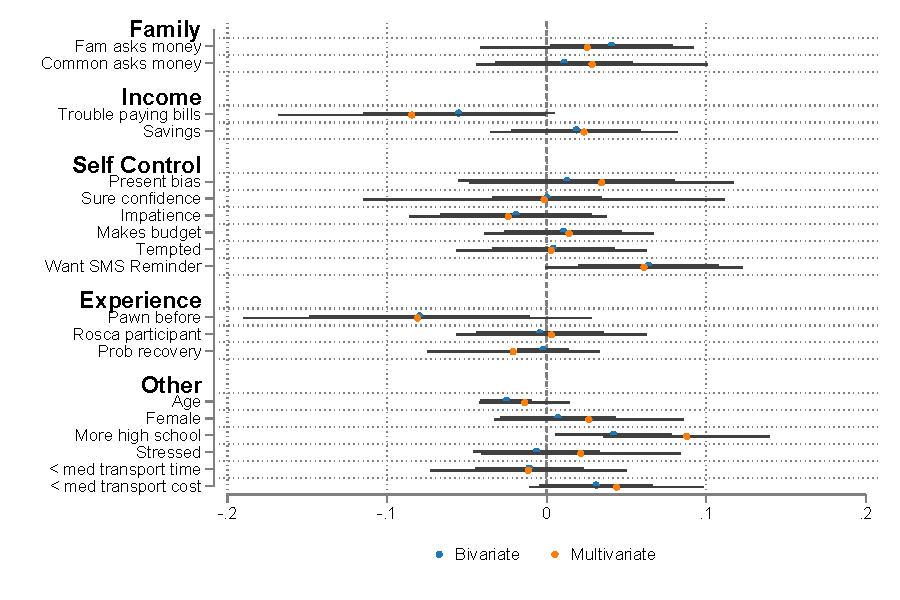
\includegraphics[width=\textwidth]{Figuras/determinants_choose_commitment.pdf}
    \end{subfigure}
    \end{center}
\footnotesize{The above figure shows the determinants in a bivariate and multivariate OLS regression of choosing commitment. Choice commitment is a binary variable equal to one, whenever subjects choose the forced commitment contract in the choice arm. }
    \label{weekly_def_rates}
%\textit{Do file: } \texttt{determinants_choice.do}       
\end{figure}


\normalsize
%Really force it to normal size and linespread
\normalsize

%%%%%%%%%%%%%%%%%%%%%%%%%%%%%%%%%%%%%%%%%%
\section{ Internal Validity}


\begin{table}[!h]
\caption{Summary statistics and Balance}
\label{SS}
\begin{center}
\resizebox{0.65\textwidth}{!}{
\footnotesize{% Table generated by Excel2LaTeX from sheet 'SS'
\begin{tabular}{lcccccccc}
\toprule
      &       &       & \multicolumn{5}{c}{Treatment arms}    &  \\
\midrule
      &       &       &       & \multicolumn{2}{c}{No Choice } & \multicolumn{2}{c}{Choice} &  \\
\midrule
\midrule
      & Overall & Pre-experiment & Control & Fee   & Promise & Fee   & Promise & p-value \\
\midrule
      & \multicolumn{8}{c}{Panel A : Administrative Data} \\
\midrule
\midrule
Loan amount  & 2197  & 2239  & 2301  & 2147  & 2133  & 2181  & 2089  & 0.32 \\
      & (25)  & (39)  & (79)  & (72)  & (74)  & (65)  & (65)  &  \\
Monday & 0.18  & 0.16  & 0.18  & 0.16  & 0.17  & 0.19  & 0.21  & 0.96 \\
      & (0.02) & (0.03) & (0.05) & (0.05) & (0.06) & (0.06) & (0.05) &  \\
Number of branch-day pawns & 34    & 36    & 31    & 31    & 32    & 37    & 34    & 0.38 \\
      & (0.82) & (1.25) & (2.2) & (2.35) & (2.38) & (2.65) & (1.76) &  \\
\midrule
Number of branch-days & -     &       & 84    & 80    & 68    & 93    & 82    &  \\
Obs   & 21808 & 8366  & 2601  & 2484  & 2156  & 3435  & 2766  &  \\
\midrule
      & \multicolumn{8}{c}{Panel B : Survey Data (conditional on pawning)} \\
\midrule
\midrule
Woman & 0.73  &       & 0.76  & 0.72  & 0.73  & 0.72  & 0.74  & 0.41 \\
      & (0.01) &       & (0.02) & (0.02) & (0.02) & (0.02) & (0.01) &  \\
Age   & 43.31 &       & 43.16 & 43.17 & 42.96 & 43.96 & 43.06 & 0.79 \\
      & (0.28) &       & (0.57) & (0.79) & (0.65) & (0.61) & (0.52) &  \\
Subjective value & 3068  &       & 3151  & 2978  & 2985  & 3114  & 3079  & 0.41 \\
      & (39)  &       & (69)  & (91)  & (76)  & (85)  & (100) &  \\
Has pawn before & 0.9   &       & 0.89  & 0.9   & 0.89  & 0.91  & 0.89  & 0.68 \\
      & (0)   &       & (0.01) & (0.01) & (0.01) & (0.01) & (0.01) &  \\
Subj. pr. of recovery & 93.14 &       & 92.74 & 92.16 & 93.6  & 93.67 & 93.3  & 0.46 \\
      & (0)   &       & (0.55) & (0.86) & (0.6) & (0.47) & (0.6) &  \\
+High-school & 0.66  &       & 0.66  & 0.67  & 0.65  & 0.67  & 0.64  & 0.74 \\
      & (0.01) &       & (0.02) & (0.02) & (0.02) & (0.02) & (0.02) &  \\
Survey response rate & 0.78  &       & 0.77  & 0.75  & 0.8   & 0.77  & 0.79  & 0.5 \\
      & (0.01) &       & (0.02) & (0.03) & (0.02) & (0.02) & (0.02) &  \\
\midrule
Obs   & 10431 &       & 2000  & 1855  & 1732  & 2652  & 2192  &  \\
\midrule
\midrule
      & \multicolumn{8}{c}{Panel C : Survey Data (unconditional)} \\
\midrule
\midrule
Woman & 0.74  & 0.75  & 0.76  & 0.72  & 0.73  & 0.72  & 0.74  & 0.32 \\
      & (0.01) & (0.01) & (0.02) & (0.02) & (0.02) & (0.02) & (0.01) &  \\
Age   & 43.24 & 43.06 & 43.2  & 43.21 & 43.01 & 44.07 & 43.07 & 0.79 \\
      & (0.21) & (0.32) & (0.56) & (0.77) & (0.66) & (0.61) & (0.51) &  \\
Subjective value & 3112  & 3192  & 3145  & 2985  & 3010  & 3111  & 3082  & 0.41 \\
      & (36)  & (75)  & (68)  & (88)  & (76)  & (84)  & (99)  &  \\
Has pawn before & 0.89  & 0.88  & 0.89  & 0.9   & 0.89  & 0.91  & 0.89  & 0.56 \\
      & (0.01) & (0.01) & (0.01) & (0.01) & (0.01) & (0.01) & (0.01) &  \\
Subj. pr. of recovery & 92.64 & 91.84 & 92.73 & 92.19 & 93.66 & 93.71 & 93.34 & 0 \\
      & (0.2) & (0.31) & (0.54) & (0.84) & (0.59) & (0.46) & (0.59) &  \\
+High-school & 0.63  & 0.6   & 0.66  & 0.67  & 0.65  & 0.66  & 0.64  & 0.01 \\
      & (0.01) & (0.01) & (0.02) & (0.02) & (0.02) & (0.02) & (0.02) &  \\
\% ended up pawning &       &       & 0.98  & 0.97  & 0.99  & 0.98  & 0.99  & 0.25 \\
\midrule
Obs   & 17546 & 6919  & 2035  & 1907  & 1757  & 2710  & 2218  &  \\
\bottomrule
\bottomrule
\end{tabular}%
}
}
\end{center}
\footnotesize {Each row in this table corresponds to a regression, where the level of observation is the individual loan originated. The dependent variables of these regressions are displayed in the first column. Each dependent variable is regressed in a multivariate OLS regression against the experimental arms indicators (control, forced commitment, choice). The table reports the coefficients on each of these indicators, as well as the p-value an F-test of the null hypothesis of equality of the three coefficients. The admin data was a very limited set of pre-determined variables. The dependent variables are: subjective value of the pawn (how much would the client be willing to sell it for (Q3), an indicator for having trouble paying bills in the last 6-months (Q28), present bias (constructed from questions Q10 and Q29 in the standard way as in \cite{Ashraf}), an indicator for whether they make expenses budget for the month ahead of time. The subjective probability of recovery was elicited a la Manski (from 0 to 100 what is the probability that you will recoup your pawn), pawned before is a dummy=1 if the client declares to have pawned before (although not necessarily with Lender $P$) age is in year, +High-school is a dummy that indicates if the client has completed high school. 
}
%\textit{Do file: } \texttt{ss\_balance.do}
\end{table}


If potential borrowers disliked being forced into a commitment contract, we would expect a lower number of pawns on branch days where only the commitment contract is available compared to control days. Table \ref{attrition_table} shows that this is not the case. There is no difference at all between the Control and Forced Commitment arm in terms of the number of pawns per branch-day. Although we cannot reject equality across the three arms (p-value=0.21), the Choice arm appears to have a somewhat larger number of borrowers than the Control and Forced arms.\footnote{p-value=0.23 and 0.12 respectively.} This seems to be due to sampling variability. Differences across arms are smaller when for medians, or when we compare the number of borrowers pawning (some borrowers pawn more than one piece). 
% Figure \ref{boxplot_attrition} shows that distribution of loans per day is comparable across arms. The only noticeable difference is that the choice arm has a few more positive outliers.\footnote{If we winzorize at the 90th percentile, the mean number of branch-day pawns becomes identical across arms.}

\begin{table}
\caption{Limited and balanced attrition}
\label{attrition_table}
\begin{center}
\footnotesize{% Table generated by Excel2LaTeX from sheet 'Attrition'
\begin{tabular}{lcccr}
\toprule
      & Control & Structure & Choice & \multicolumn{1}{c}{p-value} \\
\midrule
\midrule
Loan take-up & 0.967 & 0.955 & 0.961 & 0.82 \\
      & (0.01) & (0.01) & (0.01) &  \\
\midrule
Number of borrowers & 20.8  & 22.2  & 25.4  & 0.17 \\
      & (3.29) & (3.9) & (4.89) &  \\
\rowcolor[rgb]{ .949,  .949,  .949} \multicolumn{1}{r}{median} & 19    & 20    & 21    & 0.5 \\
\midrule
Number of pawns/borrower & 1.4   & 1.4   & 1.4   & 0.43 \\
      & (0.08) & (0.04) & (0.05) &  \\
\rowcolor[rgb]{ .949,  .949,  .949} \multicolumn{1}{r}{median} & 1.4   & 1.3   & 1.3   & 0.6 \\
\midrule
Number of pawns  & 31    & 31.3  & 37.2  & 0.24 \\
      & (5.8) & (5.6) & (7.9) &  \\
\rowcolor[rgb]{ .949,  .949,  .949} \multicolumn{1}{r}{median} & 27    & 28    & 30    & 0.46 \\
\midrule
Amt borrowed/borrower & 2266.8 & 2094  & 2115.2 & 0.18 \\
      & (101.8) & (83.7) & (99.9) &  \\
\rowcolor[rgb]{ .949,  .949,  .949} \multicolumn{1}{r}{median} & 2154.3 & 2041  & 2047.5 & 0.65 \\
\midrule
Total borrowed & 47877 & 47813 & 54780 & 0.4 \\
      & (8005) & (9436) & (12587) &  \\
\rowcolor[rgb]{ .949,  .949,  .949} \multicolumn{1}{r}{median} & 37520 & 39420 & 40850 & 0.73 \\
\midrule
Obs   & 85    & 81    & 94    &  \\
\bottomrule
\bottomrule
\end{tabular}%
}
\end{center}
\footnotesize{Each row in this table 
 corresponds to a regression. The dependent variables are: the number of pawns-loans originated per day per branch, the number of borrowers per day-branch, a variable indicating whether a person who answered the baseline survey (before knowing contract terms) ended up pawning, and an indicator of whether the person that obtained the loan answered the baseline survey. Each dependent variable is regressed in a multivariate OLS regression against the experimental arms indicators (control, forced commitment, choice). The table reports the coefficients on each of these indicators, as well as the p-value of an F-test of the null hypothesis of equality of the three coefficients. %Figure \ref{boxplot_attrition}, in the appendix shows a box-plot of the first two variables, showing the distribution across arms is balanced.
 }
%\textit{Do file: } \texttt{ss\_att.do}
\end{table}


The bottom panel of Table \ref{attrition_table} shows balance in a more focused way, given that the surveys were conducted prior to the revelation of treatment status. We find that in no arm did more than three percent of individuals who responded to the survey go on to refuse loans. That is, the overwhelming majority of potential borrowers did not leave the branch after learning which contract was on offer. Moreover, the extremely small fraction that did leave is balanced across arms.  Therefore it appears that the treatments have not induced any endogenous shifts in the composition of borrowers. 

A less critical form of attrition is differential refusal to answer the survey questions.  The survey was conducted before treatment status was revealed, and we observe loan outcomes regardless of whether the survey was conducted.  Our core experimental estimates do not use the survey data as covariates, but the analysis in Section \ref{Paternalism} is restricted to the subset of borrowers who answered at least some survey questions. The bottom row of Table \ref{attrition_table} shows that the survey response rate is broadly similar across arms (about 78 percent). 


%We now present an analysis of the extent to which the survey-responding sample is representative and balanced. Table \ref{SS_cond_survey} presents information about survey non-response. Panel A is a balance table that compares loan amount and day of the week across treatment arms for the subset of borrowers who responded to at least one survey question. The p-values in the fourth column are for the F-test of no difference of means across treatment arms. Panel B presents response-rates by question for each arm of the experiment, along with p-values for the F-test of no difference in question-specific response rates across treatment arms. This panel uses data from participants who answered at least one survey question and went on to pawn on the same day as their survey response. From the table, we see that loan amount and weekday are balanced across treatment arms among survey respondents and that response rates are likewise stable across treatment arms.

% Table \ref{TUT_cond_survey} shows how the estimated TUT effect changes if we restrict our estimation sample based on survey response.
% The first row of the table presents TUT results for the financial cost outcome, while the second presents corresponding results for the APR outcome.
% In each row, column (1) presents the full-sample TUT estimate and standard error while the remaining columns restrict the sample to borrowers who answered a particular survey question or set of questions.
% For example, column (4) presents results for borrowers who answered the two questions needed to compute our measure of ``present bias'' discussed in the next paragraph, while column (9) present results restricted to participants who disclosed their sex. 
% As seen from the table, our TUT estimates are quite stable across sub-samples defined by survey response.
% In each case they are positive and of the same magnitude as the corresponding full-sample estimate, although statistical significance varies depending on the size of the corresponding sub-sample. 
% For these reasons, we are comfortable relying on data for survey respondents in the empirical exercises that follow.
% In exercises that rely on a single survey question, we use data for every borrower who answered that question.
% In the random forest exercises described below, we use data for every borrower who answered at least one survey question.



% \begin{table}[H]
% \caption{Survey Non-response: TUT estimates for respondents to each survey question.}
% \label{TUT_cond_survey}
% \begin{center}
% \footnotesize{% Table generated by Excel2LaTeX from sheet 'tut_cond_survey'
\begin{tabular}{lcccccccccc}
\toprule
      & Full-sample & Subjective value & Trouble paying bills & Present bias & Makes budget & Subj. pr. of recovery & Pawn before & Age   & Woman & + High-school \\
\midrule
      & (1)   & (2)   & (3)   & (4)   & (5)   & (6)   & (7)   & (8)   & (9)   & (10) \\
\midrule
\midrule
FC benefit TuT & 10.3*** & 10.4*** & 11.3*** & 12.0*** & 10.3*** & 11.2*** & 10.4*** & 10.9*** & 11.4*** & 10.8*** \\
      & (2.46) & (2.36) & (2.59) & (2.64) & (2.69) & (2.29) & (2.68) & (2.90) & (2.92) & (2.85) \\
      &       &       &       &       &       &       &       &       &       &  \\
\midrule
      & (11)  & (12)  & (13)  & (14)  & (15)  & (16)  & (17)  & (18)  & (19)  & (20) \\
\midrule
\midrule
Apr \% benefit & 189.1*** & 185.6*** & 143.7** & 183.9** & 153.9** & 181.2*** & 140.5** & 159.7** & 137.2** & 128.0* \\
      & (50.9) & (58.0) & (67.6) & (81.9) & (69.8) & (60.7) & (68.6) & (74.6) & (69.2) & (72.6) \\
      &       &       &       &       &       &       &       &       &       &  \\
\midrule
Observations & 6304  & 4465  & 2948  & 2613  & 3433  & 4625  & 3468  & 3393  & 3677  & 3352 \\
\bottomrule
\bottomrule
\end{tabular}%
}
% \end{center}
% \footnotesize{Some borrowers did not respond to our survey; others only completed part of the survey.
% This table computes the TUT effect for a number of sub-groups by survey response, and compares them against the overall TUT effect.
% The top panel uses financial cost as the outcome variable, while the bottom panel uses APR.
% Each group is defined by the borrowers who responded to a particular \emph{subset} of the survey questions. 
% For example, column (4) computes TUT effects for the subgroup of borrowers who responded to the two questions needed to compute our measure of present bias, while column (8) computes the TUT for the subgroup of borrowers who provided their age.
% The bottom row of the table counts the number of borrowers in each category.
% TUT estimates are quite stable across sub-groups and generally similar to the full-sample estimates.
% Because standard errors increase as sample size falls, some of the sub-group estimates are not statistically significant.}
% %\textit{Do file: } \texttt{tut_cond_survey.do}
% \end{table}


\section{ Main treatment effects: Additional material}


\begin{figure}[H]
    \caption{Determinants of choice.}
    \begin{center}
    \begin{subfigure}{0.65\textwidth}
        \centering
        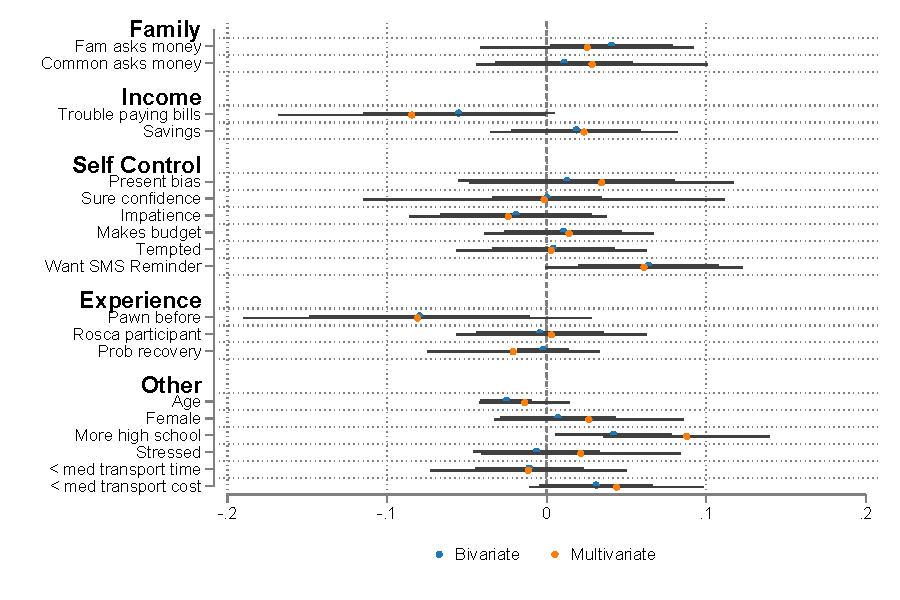
\includegraphics[width=\textwidth]{Figuras/determinants_choose_commitment.pdf}
    \end{subfigure}
    \end{center}
\footnotesize{The above figure shows the determinants in a bivariate and multivariate OLS regression of choosing commitment. Choice commitment is a binary variable equal to one, whenever subjects choose the forced commitment contract in the choice arm. }
    \label{determinants_choose}
%\textit{Do file: } \texttt{determinants_choice.do}       
\end{figure}


\subsection{Intermediate Outcomes}

\begin{landscape}
    
\begin{table}[!h]
\caption{Effects on intermediate outcomes}
\label{mechanisms}
\begin{center}

\scriptsize{% Table generated by Excel2LaTeX from sheet 'mechanism'
\begin{tabular}{lccccccc}
\toprule
      & \% of payment in 1st visit & $\Pr($Recovery in 1st visit) & \% of payment & $\Pr($+ payment \& default) & \% of pay $|$ def  & $\Pr($Selling pawn) & $\Pr($Selling pawn $|$ def) \\
\midrule
\midrule
      & (1)   & (2)   & (3)   & (4)   & (5)   & (6)   & (7) \\
\midrule
\midrule
Forced commitment & 7.92*** & 0.079*** & 9.43*** & -0.070*** & -3.90*** & 0.0050 & 0.14*** \\
      & (2.78) & (0.026) & (2.62) & (0.015) & (1.26) & (0.021) & (0.034) \\
Choice commitment & -0.97 & -0.010 & 1.40  & -0.026* & -1.75* & 0.0035 & 0.049* \\
      & (2.20) & (0.022) & (2.36) & (0.013) & (1.00) & (0.019) & (0.029) \\
      &       &       &       &       &       &       &  \\
\midrule
Observations & 6304  & 6304  & 6304  & 6304  & 2488  & 6304  & 2488 \\
R-squared & 0.014 & 0.016 & 0.015 & 0.011 & 0.022 & 0.016 & 0.033 \\
Control Mean & 44.7  & 0.30  & 67.2  & 0.12  & 9.46  & 0.31  & 0.72 \\
\midrule
\midrule
      &       &       &       &       &       &       &  \\
\midrule
      & Days to 1st payment & \# of visits & \# of visits $|$ recovery & \# of visits $|$ def & Loan duration (days) & Loan duration $|$ recovery &  \\
\midrule
\midrule
      & (8)   & (9)   & (10)  & (11)  & (12)  & (13)  &  \\
\midrule
\midrule
Forced commitment & -13.8*** & -0.031 & -0.19*** & 0.062 & -27.9*** & -17.9*** &  \\
      & (1.61) & (0.049) & (0.049) & (0.053) & (4.35) & (3.88) &  \\
Choice commitment & -3.51** & 0.085 & -0.077* & 0.13** & -0.18 & -1.35 &  \\
      & (1.57) & (0.053) & (0.041) & (0.063) & (4.33) & (4.19) &  \\
      &       &       &       &       &       &       &  \\
\midrule
Observations & 4412  & 6304  & 2488  & 3031  & 6304  & 3031  &  \\
R-squared & 0.055 & 0.022 & 0.025 & 0.018 & 0.054 & 0.041 &  \\
Control Mean & 82.8  & 1.14  & 0.39  & 1.44  & 136.6 & 103.9 &  \\
\bottomrule
\bottomrule
\end{tabular}%
}

\end{center}
\footnotesize{This table explores treatment effects in ``intermediate variables''. Each column represents regression output for different dependent variables following equation (\ref{basic_reg}). Panel A focuses on variables related to the speed of payment. While Panel B focuses on variables related to default, and Panel C related to visits. 
% The outcome variables are as follows:  number of days elapsed between origination and first payment (col 1); percentage of the loan paid in the first payment (col 2); probability of recovery in the first visit (col 3); loan duration is the number of days the borrower took to payoff her loan for those that recover, the number of days until default for those that default, and the maximum number of days we observe them in the sample for those that have not recovered or defaulted (col 4); loan duration conditional on recovery; an indicator for paying a positive amount towards recovery but nonetheless losing the pawn (col 6); the percentage or the loan paid, conditional on defaulting --`wasted payments' (col 7). Column 8 uses the phrase `selling the pawn' for a dummy variable indicating the borrower did not pay any amount towards recovery and lost the pawn. Moreover, (col 9) shows that treatment effects are concentrated in the intensive margin as treatment does not affect the fraction of clients who pay a positive amount towards pawn recovery. The dependent variable in column 10 is the number of day-visits to the branch (measured by the existence of transactions that day associated with our particular pawn), while column 11 conditions on borrowers that lost the pawn.
Each regression includes branch and day-of-week FE. Standard errors are clustered at the branch-day level.}
%\textit{Do file: } \texttt{mechanisms.do}
\end{table}
\end{landscape}

\normalsize
%Really force it to normal size and linespread
\normalsize


\subsection{Censoring} \label{App_censoring}


Some loans in our sample are ``censored'' in that they continue beyond our observation period.  For these loans, we do not know whether the borrower ultimately defaulted or recovered her pawn.   We have also shown that one effect of the forcing arm is to accelerate repayment, meaning that it is less likely for loans in this arm to be censored.  This issue is illustrated in Figure \ref{survival_graph}, which shows the CDF of loan completion (either default or recovery in Panel (a)) and loan recovery (Panel (b)) by the number of days since first pawn.  Two features of these graphs are salient for our analysis.  The first is the extent to which loan outcomes are observed more quickly in the forced commitment arm.  This is primarily due to the substantially higher rate of repayment of Forced Commitment loans at 120 days (15 pp higher than the other arms).  The second is the very low rate at which loans are recovered in any arm after 120 days.  In the 180-320 day window loans are largely dormant, suggesting that many of the censored loans will in fact end in default.

The confluence of censoring and a treatment effect on censoring is potentially problematic from an experimental point of view.  The approach taken in the headline results is a conservative one in that it inherently assumes that all of the loans outstanding at the end of the observation window will be repaid, making it so that the acceleration of payment observed in the Forced arm does not translate mechanically into the that treatment decreasing default.  Nonetheless, to be certain that this issue is not driving our results we conduct a bounding exercise to understand how large the effects of this problem can possibly be.  

One way of considering the effect that this issue could have on our results is to make extreme assumptions about the outcome of these loans in the treatment and control so as to bound the possible influence of censoring. In Table \ref{bounding_censoring} we compare the Forced and Control arms, bounding the censoring issue by reversing assumptions about the outcome of censored loans in the treatment versus the control.   Panel B provides the lower bound for the treatment effect (closest to zero) by assuming censored control loans are always repaid and treatment loans never are; even in this lower-bound case the treatment effect is cost-reducing and significant at the 1\% significance level and indeed the magnitude of this lower bound estimate is only 6\% closer to zero than our headline result.   Panel C estimates the upper bound by making the reverse assumption.  Comfortingly, even with these extreme assumptions the significance on the main treatment effects never flips and treatment effects on financial cost and interests payments remain negative and significant in all scenarios.  So there appears to be no scope for the censoring issue to overturn our main results. 

Finally, Panel E of this table conducts a logit prediction model that uses all of the available information on loans that were completed to predict the outcome of loans that were not.  This is a ``best guess'' of the outcome on censored loans.  Using this prediction, we replicate the main experimental results and find that the treatment effect on financial cost increases from -204 (main results) to -264 (censored loans predicted), and the APR from -11\% to -17\%.  Hence, while the censoring issue does have an effect on the magnitude of our estimated treatment effects, these  checks confirm that (a) the core results are fully robust to censoring, and (b) the headline approach that we take to the issue is conservative and likely understates the true magnitude of impacts.





\begin{table}[H]
\caption{Bounding censoring} 
\label{bounding_censoring}
\begin{center}
\resizebox{0.75\textwidth}{!}{
\footnotesize{% Table generated by Excel2LaTeX from sheet 'censoring_imp'
\begin{tabular}{lcccccc}
\toprule
      & FC    & Interest pymnt & Principal pymnt & Lost pawn value & Default & APR \\
\midrule
      & \multicolumn{6}{c}{Panel A : $\quad$ Control  = 0           $\quad\quad$                  Forced Commitment = 0} \\
\midrule
\midrule
      & (1)   & (2)   & (3)   & (4)   & (5)   & (6) \\
\midrule
\midrule
Forced commitment  & -236.0*** & -191.7*** & -0.63 & -75.9** & -0.064*** & -0.14*** \\
      & (48.1) & (37.6) & (3.01) & (30.5) & (0.023) & (0.022) \\
      &       &       &       &       &       &  \\
\midrule
Observations & 3724  & 3724  & 3724  & 3724  & 3724  & 3724 \\
R-sq  & 0.016 & 0.025 & 0.004 & 0.012 & 0.019 & 0.043 \\
Control Mean & 989.9 & 593.4 & 5.96  & 396.5 & 0.44  & 0.61 \\
\midrule
\midrule
      &       &       &       &       &       &  \\
\midrule
      & \multicolumn{6}{c}{Panel B : $\quad$ Control  = 0         $\quad\quad$                    Forced Commitment = 1} \\
\midrule
\midrule
      & (7)   & (8)   & (9)   & (10)  & (11)  & (12) \\
\midrule
\midrule
Forced commitment  & -191.2*** & -207.7*** & 1.17  & -15.1 & 0.0083 & -0.076*** \\
      & (49.7) & (37.4) & (3.45) & (31.2) & (0.024) & (0.026) \\
      &       &       &       &       &       &  \\
\midrule
Observations & 3724  & 3724  & 3724  & 3724  & 3724  & 3724 \\
R-sq  & 0.013 & 0.026 & 0.004 & 0.009 & 0.014 & 0.023 \\
Control Mean & 989.9 & 593.4 & 5.96  & 396.5 & 0.44  & 0.61 \\
\midrule
\midrule
      &       &       &       &       &       &  \\
\midrule
      & \multicolumn{6}{c}{Panel C : $\quad$ Control  = 1        $\quad\quad$                     Forced Commitment = 0} \\
\midrule
\midrule
      & (13)  & (14)  & (15)  & (16)  & (17)  & (18) \\
\midrule
\midrule
Forced commitment  & -319.0*** & -140.4*** & -2.33 & -210.3*** & -0.21*** & -0.24*** \\
      & (50.9) & (34.1) & (3.16) & (30.3) & (0.023) & (0.027) \\
      &       &       &       &       &       &  \\
\midrule
Observations & 3724  & 3724  & 3724  & 3724  & 3724  & 3724 \\
R-sq  & 0.021 & 0.020 & 0.004 & 0.021 & 0.053 & 0.061 \\
Control Mean & 1069.2 & 545.9 & 7.69  & 523.3 & 0.57  & 0.70 \\
\midrule
\midrule
      &       &       &       &       &       &  \\
\midrule
      & \multicolumn{6}{c}{Panel D : $\quad$ Control  = 1       $\quad\quad$                      Forced Commitment = 1} \\
\midrule
\midrule
      & (19)  & (20)  & (21)  & (22)  & (23)  & (24) \\
\midrule
\midrule
Forced commitment  & -274.2*** & -156.3*** & -0.53 & -149.6*** & -0.13*** & -0.17*** \\
      & (52.5) & (33.8) & (3.58) & (31.1) & (0.024) & (0.030) \\
      &       &       &       &       &       &  \\
\midrule
Observations & 3724  & 3724  & 3724  & 3724  & 3724  & 3724 \\
R-sq  & 0.017 & 0.021 & 0.003 & 0.013 & 0.028 & 0.032 \\
Control Mean & 1069.2 & 545.9 & 7.69  & 523.3 & 0.57  & 0.70 \\
\midrule
\midrule
      &       &       &       &       &       &  \\
\midrule
      & \multicolumn{6}{c}{Panel E : $\quad$ Prediction with lasso-logit model} \\
\midrule
\midrule
      & (25)  & (26)  & (27)  & (28)  & (29)  & (30) \\
\midrule
\midrule
Forced commitment  & -264.9*** & -169.6*** & -1.43 & -127.4*** & -0.12*** & -0.17*** \\
      & (53.8) & (37.2) & (3.52) & (33.1) & (0.025) & (0.028) \\
Choice commitment & -42.4 & -29.1 & -2.66 & -14.6 & -0.017 & 0.0026 \\
      & (56.9) & (41.8) & (3.24) & (34.9) & (0.024) & (0.029) \\
      &       &       &       &       &       &  \\
\midrule
Observations & 6304  & 6304  & 6304  & 6304  & 6304  & 6304 \\
R-sq  & 0.018 & 0.022 & 0.002 & 0.010 & 0.016 & 0.042 \\
Control Mean & 1034.5 & 563.4 & 7.69  & 471.2 & 0.52  & 0.66 \\
\bottomrule
\bottomrule
\end{tabular}%
}
}
\end{center}
 
\end{table}
 \footnotesize{ Given the censored loans, i.e. loans that have not finished by the end of the observation period, we estimate `a la Manski' bounds for these loans, meaning that we impute all loans to either \emph{default}$=1$ or \emph{recovery}$=0$ depending on the treatment arm. Different panels perform different imputations for the censored loans for all possible combinations for the imputation, and computes the ATE for the same outcomes of Table \ref{main_impact_table}. Panel A, for instance, assumes that all outstanding loans are fully payed. Panel B is the most conservative imputation since it assumes all outstanding loans in the control arm are payed, while all the outstanding loans in the forced commitment arm default. Panel C, on the other hand, is the most optimistic scenario opposite to that of Panel B. Panel D assumes all remaining loans default. The last panel makes the imputation to the censored loans according to the best prediction using a piecewise lasso logit model for default. In concrete, we build two logit models with lasso regularization, depending whether the loan duration is less than 220 days (two cycles) or more than 220 days. For prediction we use the former whenever the last recorded payment was done within 220 days, and the latter otherwise. Both models includes loan characteristics (loan size, branch), and payment behavior (loan duration so far, days to first payment, \% of first payment, \% of payments at 30, 60, 90, and 105 days, and \% of interest payed at 105 days), but the latter model also includes \% of payments at 150, 180, and 210 days. This predictive model achieves an accuracy rate of 92\% both in-sample and out-of-sample.
 Note that in all panels we maintain significant results for Financial Cost as dependent variable, while only in the most conservative scenario (Panel B) we lose significance for the APR outcome. }


% \begin{figure}[H]
    
%     \begin{center}
%    % \begin{subfigure}{0.49\textwidth}
%    % \caption{Significance area for APR}
%    %      \centering
%    %      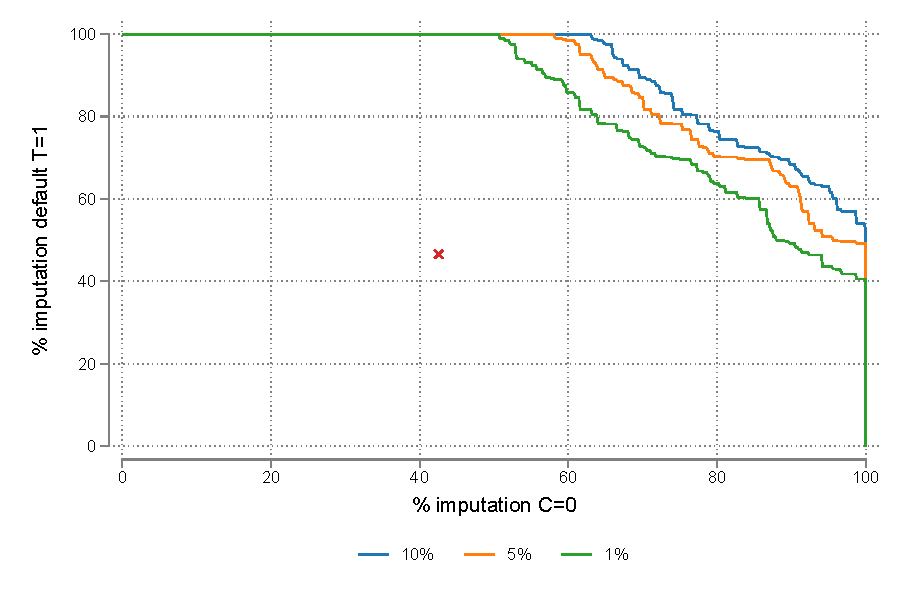
\includegraphics[width=\textwidth]{Figuras/frontera_sig_apr.pdf}
%    %  \end{subfigure}     
%    %  \begin{subfigure}{0.49\textwidth}
%    % \caption{Significance area for Default }
%         \centering
%         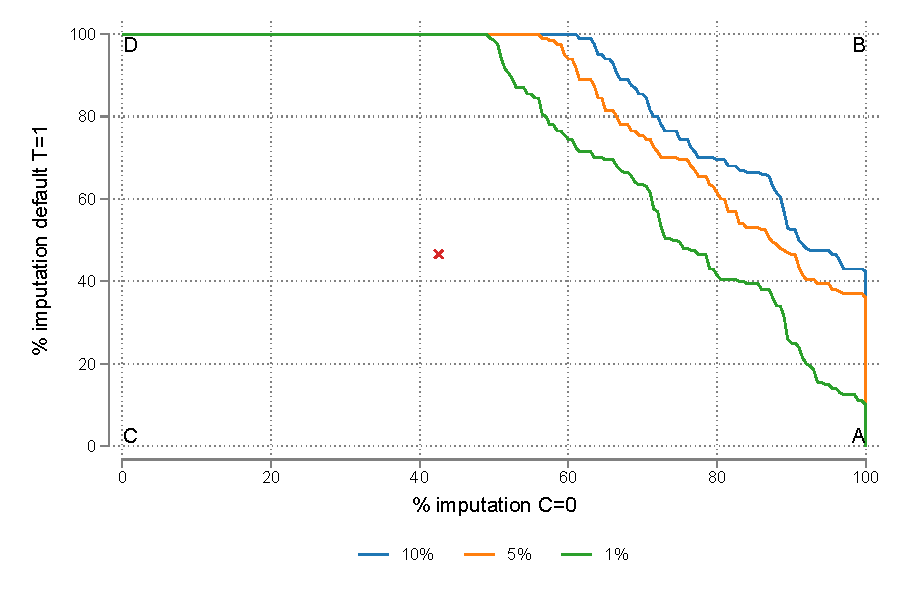
\includegraphics[width=0.5\textwidth]{Figuras/frontera_sig_def_imp.pdf}
%     % \end{subfigure} 
%     \end{center}
%  \caption{Interpolation on bounding censoring for Default. This figure aims to answer the following question: For how many loans in the control arm can we impute recovery, and for how many in the treatment arm can we impute default and still have significance?
%      This figure shows exactly the boundary separating significance when we vary the percentage of imputed censored loans with recovery and default respectively for control and treatment. Each corner in the square will correspond to one of the panels from the Table \ref{bounding_censoring}. For instance, the origin is the best-case scenario (Panel C) and the point (100,100) (Panel B) is the worst-case scenario. Thus we can think of this graph as an `interpolation' from the four extreme cases. The `x' indicates the proportions imputed by the lasso logit model, and the different lines correspond to setting different significance levels. We do not include the plot for APR nor financial cost, since for any imputation we still have significant results.}
%  \label{interpolation_censoring_imp}
%      %\textit{Do file: }  \texttt{interpolation_censoring_imp.do}
% \end{figure}





\begin{figure}[H]
\caption{Survival graph.}
    \begin{center}
   \begin{subfigure}{0.49\textwidth}
   \caption{Ended contract}
        \centering
        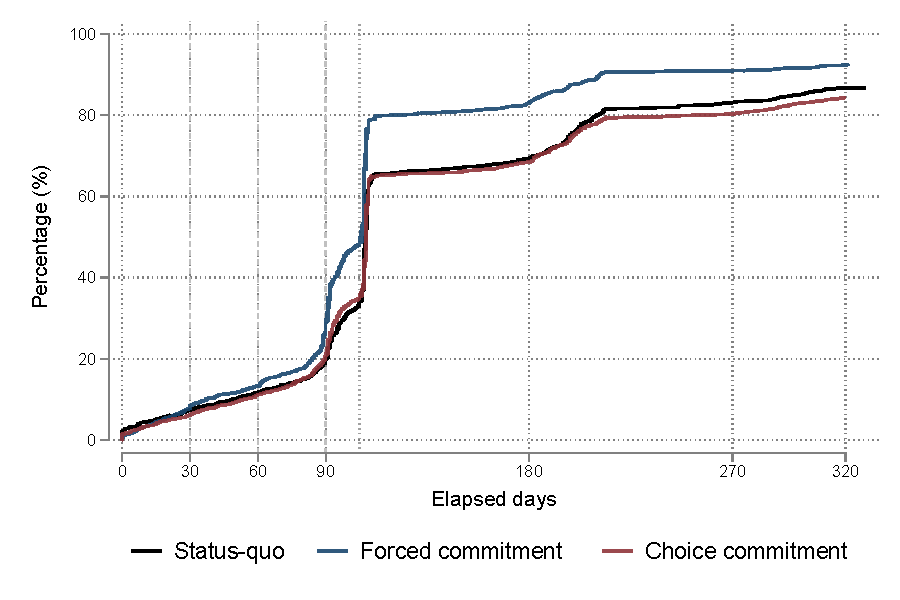
\includegraphics[width=\textwidth]{Figuras/survival_graph_ended.pdf}
    \end{subfigure} 
   \begin{subfigure}{0.49\textwidth}
   \caption{Recovery}
        \centering
        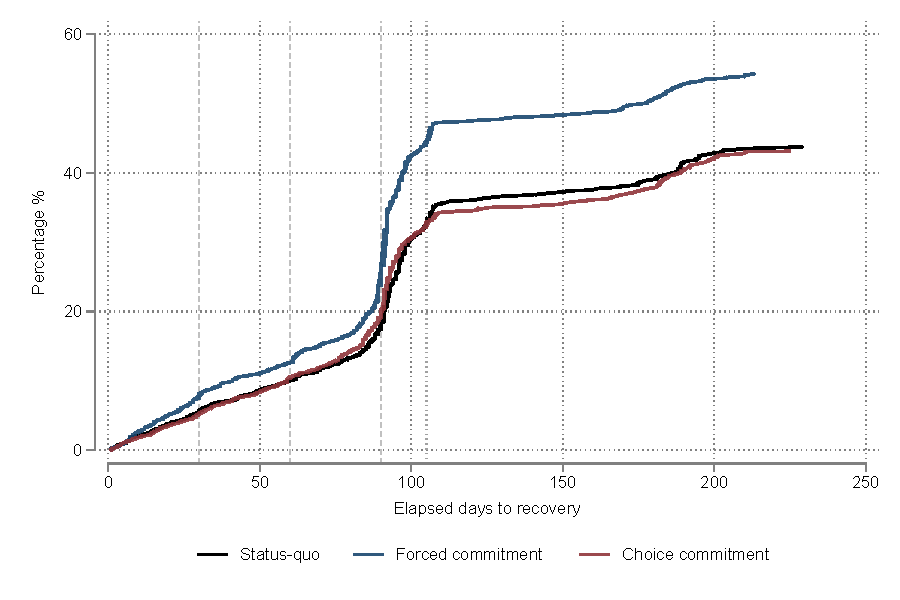
\includegraphics[width=\textwidth]{Figuras/survival_graph_unpledge.pdf}
    \end{subfigure}     
    \end{center}
      \footnotesize{This Figure shows the CDF of loan completion either default or recovery in Panel (a), or loan recovery in Panel (b), by the number of days since first pawn.}
      \label{survival_graph}
     %\textit{Do file: }  \texttt{survival\_graph.do}
\end{figure}

% \begin{figure}[H]
%     \begin{center}
%    \begin{subfigure}{0.49\textwidth}
%         \caption{Unconditional}
%         \centering
%         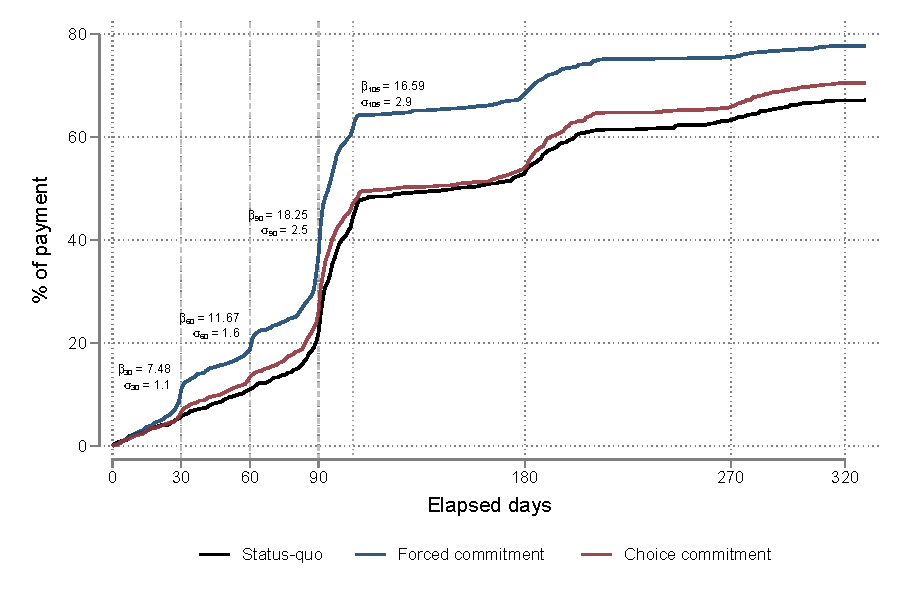
\includegraphics[width=\textwidth]{Figuras/cumulative_porc_pay_time.pdf}
%     \end{subfigure} 
%    \begin{subfigure}{0.49\textwidth}
%         \caption{Conditional on default}
%         \centering
%         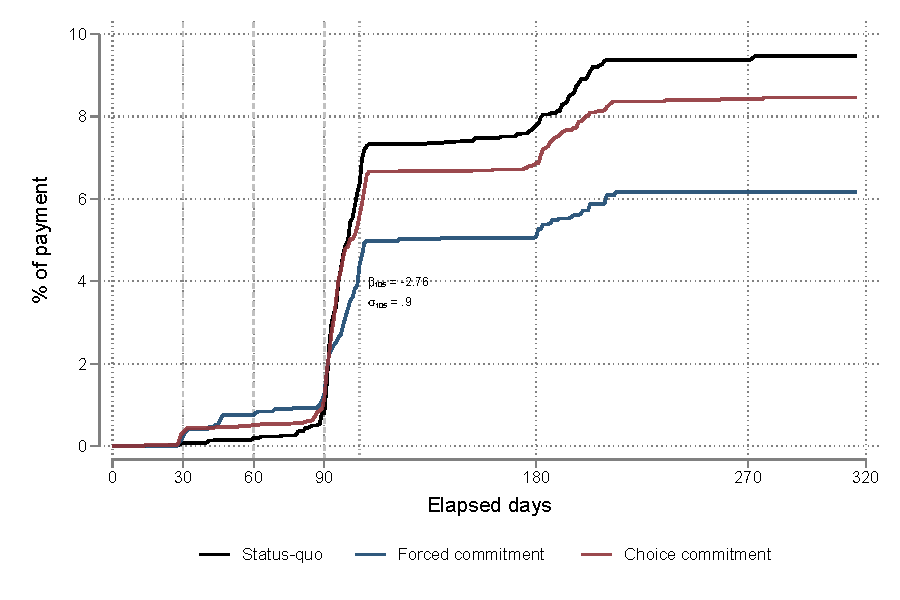
\includegraphics[width=\textwidth]{Figuras/cumulative_porc_pay_time_default.pdf}
%     \end{subfigure}     
%     \end{center}
%     \caption{\% of payment over time. This Figure shows the accumulated percentage of recovery in time by treatment arm. }
%     \label{porc_payment_over_time}
%      %\textit{Do file: }  \texttt{cumulative\_porc\_pay\_time.do}
% \end{figure}




\subsection{Robustness accounting for other costs}

\begin{table}[!h]
\caption{Effects on more comprehensive cost measures}
\label{table_robustness_fc}
\begin{center}
\resizebox{0.9\textwidth}{!}{
\footnotesize{% Table generated by Excel2LaTeX from sheet 'fc_robustness'
\begin{tabular}{lccccc}
\toprule
      & FC    & FC (subj.value) & FC +  tc & FC - interest & FC (subj.value) + tc - int \\
\midrule
      & (1)   & (2)   & (3)   & (4)   & (5) \\
\midrule
\midrule
Forced commitment & -204.0*** & -299.9*** & -207.7*** & -98.5*** & -146.3** \\
      & (48.1) & (83.3) & (49.0) & (36.7) & (72.8) \\
Choice comitment & -38.9 & -56.4 & -32.6 & -30.7 & -25.3 \\
      & (49.8) & (83.5) & (50.9) & (39.2) & (74.4) \\
      &       &       &       &       &  \\
\midrule
Observations & 6304  & 6304  & 6304  & 6304  & 6304 \\
R-squared & 0.013 & 0.009 & 0.014 & 0.005 & 0.006 \\
Control Mean & 942.4 & 1389.9 & 1026.1 & 480.7 & 927.7 \\
\midrule
\midrule
      &       &       &       &       &  \\
\midrule
      & APR   & APR (subj.value) & APR +  tc & APR - interest & APR (subj.value) + tc - int \\
\midrule
      & (6)   & (7)   & (8)   & (9)   & (10) \\
\midrule
\midrule
Forced commitment & -0.11*** & -0.22*** & -0.13*** & -0.062*** & -0.097** \\
      & (0.019) & (0.051) & (0.028) & (0.019) & (0.044) \\
Choice comitment & -0.0086 & -0.053 & -0.0035 & -0.031* & -0.043 \\
      & (0.019) & (0.045) & (0.028) & (0.018) & (0.040) \\
      &       &       &       &       &  \\
\midrule
Observations & 6304  & 6304  & 6304  & 6304  & 6304 \\
R-squared & 0.031 & 0.011 & 0.027 & 0.008 & 0.007 \\
Control Mean & 0.57  & 1.12  & 0.72  & 0.31  & 0.84 \\
\bottomrule
\bottomrule
\end{tabular}%
}
}
\end{center}
 \footnotesize{ This table augments the measure of financial cost presented in Table \ref{main_impact_table} with measures of transaction costs, subjective costs, and adjustments for liquidity costs. Panel A reports financial cost in pesos, while Panel B shows APR. Columns (1) and (6) replicate our previous results for comparability. Columns (2) and (7) of Table \ref{table_robustness_fc} use the subjective value of the pawn reported by the borrower rather than its appraised value. Columns (3) and (8) adjust for self-reported transport costs per visit plus an entire day's wage, both multiplied by the number of visits that each individual made.\footnote{For clients who did not complete the individual survey, we adjust using the mean self-reported transport cost among respondents of the respective branch.} Columns (4) and (9) adjust to consider the liquidity cost. Finally, columns (5) and (10) include all three changes together. The main takeaway from the table is that results are quite robust to including a much expanded measure of costs. Each regression includes branch and day-of-week FE. Standard errors are clustered at the branch-day level.}
%\textit{Do file: } \texttt{fc\_robustness.do}
\end{table}

\newpage 

\normalsize

%Really force it to normal size and linespread
\normalsize


\section{ Alternative explanations}
\subsection{Learning}


Table \ref{learning_table} presents information about borrowers' \emph{future} pawning behavior as a function of treatment assignment. Column (1) considers the 228 clients who returned only a second time to pawn again at a day/branch that was randomly assigned to the choice arm. Each of the two rows in this column presents a difference of mean commitment take-up rates, and associated standard error. The first row compares those who were \emph{initially} assigned to forced commitment against those where were assigned to control; the second row compares those who were initially assigned to the choice commitment arm to those who were assigned to the other two arms. In each case, there is no statistically discernible difference in the rates of commitment take-up. Granted, this is a selected sample because the decision to pawn again is potentially endogenous to the initial treatment allocation. For this reason, Column (2) considers the full sample of 4441 borrowers by re-defining the outcome variable to be an indicator for returning to pawn again at a branch/day when commitment was offered \emph{and} choosing commitment. This composite outcome variable is not subject to the sample selection problem (although it is directly driven by the decision to repeat borrow). The comparison in the two rows remains the same: forced commitment versus control in row one and choice commitment versus forced arms in row two. Again, there is no statistically discernible difference in commitment take-up rates in either row. While these exercises cannot completely exclude the possibility that learning plays a role, they provide no indication that the lack of voluntary compliance is simply a matter of inexperience with commitment.



\begin{table}[H]
        \caption{Effect of Prior Assignment on Subsequent Choice}
    \label{learning_table}
\begin{center}
\footnotesize{% Table generated by Excel2LaTeX from sheet 'learning_exp'
\begin{tabular}{lccc|ccc}
\toprule
      & \multicolumn{3}{c|}{Choose Fee} & \multicolumn{3}{c}{Choose Promise} \\
\midrule
      & (1)   & (2)   & (3)   & (4)   & (5)   & (6) \\
\midrule
\midrule
Fee-forcing (FF) & 0.078 & 0.016 & 0.090 & 0.094 & -0.029 & 0.17 \\
      & (0.076) & (0.087) & (0.12) & (0.11) & (0.15) & (0.16) \\
Fee-promise (FP) & 0.085 & 0.033 & 0.19  & -0.030 & -0.082 & -0.14 \\
      & (0.11) & (0.034) & (0.17) & (0.18) & (0.28) & (0.20) \\
Choice/SQ (CSQ) & 0.069 & 0.10  & 0.14  & 0.085 & 0.12  & 0.17 \\
      & (0.063) & (0.063) & (0.13) & (0.071) & (0.11) & (0.11) \\
Choice/Fee (CF) & -0.049 & -0.094 & -0.017 & -0.20 & 0.26  & -0.28 \\
      & (0.10) & (0.10) & (0.14) & (0.16) & (0.29) & (0.22) \\
Decision epoch 2 (D2) &       & -0.16 &       &       & -0.21 &  \\
      &       & (0.16) &       &       & (0.22) &  \\
Decision epoch 3 D(3) &       & 0.037 &       &       & 0.027 &  \\
      &       & (0.034) &       &       & (0.15) &  \\
FF\#D2 &       & 0.17  &       &       & 0.46  &  \\
      &       & (0.20) &       &       & (0.28) &  \\
FF\#D3 &       & -0.017 &       &       & -0.14 &  \\
      &       & (0.081) &       &       & (0.27) &  \\
FP\#D2 &       & 0.49  &       &       & 0.30  &  \\
      &       & (0.29) &       &       & (0.34) &  \\
FP\#D3 &       & -0.30 &       &       & -0.016 &  \\
      &       & (0.27) &       &       & (0.39) &  \\
CSQ\#D2 &       & 0.096 &       &       & 0.12  &  \\
      &       & (0.16) &       &       & (0.24) &  \\
CSQ\#D3 &       & -0.16 &       &       & -0.044 &  \\
      &       & (0.084) &       &       & (0.18) &  \\
CF\#D2 &       & 0.062 &       &       & -0.38 &  \\
      &       & (0.29) &       &       & (0.29) &  \\
CF\#D3 &       & 0.071 &       &       & -0.39 &  \\
      &       & (0.16) &       &       & (0.36) &  \\
Default (Def) &       &       & 0.15  &       &       & 0.12 \\
      &       &       & (0.13) &       &       & (0.14) \\
FF\#Def &       &       & 0.19  &       &       & -0.17 \\
      &       &       & (0.25) &       &       & (0.20) \\
FP\#Def &       &       & -0.23 &       &       & 0.13 \\
      &       &       & (0.18) &       &       & (0.24) \\
CSQ\#Def &       &       & -0.13 &       &       & -0.17 \\
      &       &       & (0.13) &       &       & (0.17) \\
CF\#Def &       &       & 0.031 &       &       & 0.11 \\
      &       &       & (0.14) &       &       & (0.30) \\
      &       &       &       &       &       &  \\
\midrule
Observations & 150   & 150   & 150   & 152   & 152   & 152 \\
R-sq  & 0.720 & 0.768 & 0.763 & 0.640 & 0.681 & 0.651 \\
DepVarMean & \multicolumn{3}{c|}{0.053} & \multicolumn{3}{c}{0.20} \\
Individual FE & \checkmark & \checkmark & \checkmark & \checkmark & \checkmark & \checkmark \\
\bottomrule
\bottomrule
\end{tabular}%
}
\end{center}
 \footnotesize{Column (1) reports results for the 228 borrowers who returned to pawn again at a day/branch that was randomly assigned to the choice arm, enabling us to observe whether they chose commitment or the status quo contract.
Each row presents a difference in mean commitment take-up rates and associated standard errors.
The first row (ATE) compares borrowers who were initially assigned to forced commitment against those were assigned to the control condition.
The second row (ITT) compares borrowers who were initially assigned to the choice commitment condition to those who were not.
Whereas column (1) conditions on the (endogenously) selected sample of borrowers who return to pawn again, column (2) considers the full sample by re-defining the ``outcome'' to be an indicator for whether a borrower pawned again on a day when choice was offered \emph{and} chose commitment.}

%This table explores learning by focusing on a subsample of borrowers in the experiment and observing their subsequent behavior. Column 1 conditions the sample on borrowers who (a) pawned during the experiment a subsequent time after being assigned to control, forced commitment or choice (the regressors), and (b) when pawning again they went to a branch day when (randomly) choice was available, thus enabling us to observe if they chose the commitment contract or the status quo.  in this sample it estimates a linear probability model where the dependent variable is equal to one if the borrower chose the commitment contract in that subsequent `choice' occasion and zero otherwise. The regressors are indicators for the treatment arms in their first pawn in the experiment. Column 1 conditions the sample on the (endogenous) event of pawning again. Column 2 does not condition the sample, but instead defined the dependent variable as equal to one \hl{if the borrower pawned subsequently and choice was available that day and chose commitment, and zero otherwise.}

\end{table}
\normalsize
%Really force it to normal size and linespread
\normalsize


\newpage 

\subsection{Discount rates}


\begin{figure}[!h]
  \caption{Financial benefit TUT effect for different discount rates.}
    \begin{center}
        \centering
        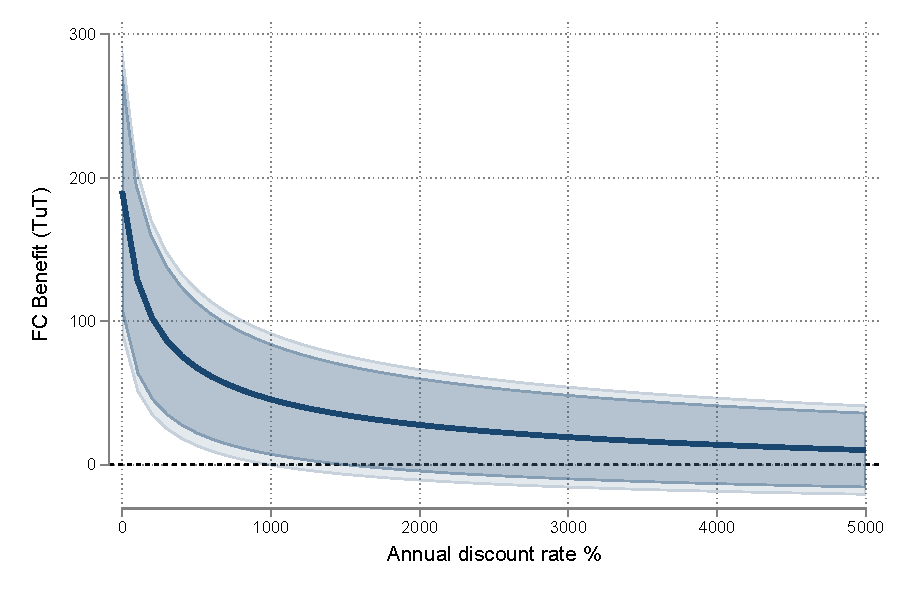
\includegraphics[width=0.65\textwidth]{Figuras/discount_effect_tut.pdf}
    \end{center}
       \footnotesize{This Figure re-estimates the treatment on the untreated (TUT) effect from Table \ref{tot_tut}, introducing a daily discount factor in the definition of financial benefit.  At a given annual discount rate in percentage points (x-axis) the solid line gives the adjusted TUT and the shaded regions 90\% \& 95\% confidence bands. A discount factor of one corresponds to the estimate from Table \ref{tot_tut}. As seen from the figure, borrowers would need to face unrealistically large discount rates to reverse our headline result of a large, positive, and statistically significant TUT effect.}
        \label{fc_discount_rates}
     %It estimates the effect of the treatment arms  for different discount factors, where a discount factor of 1 corresponds exactly to the estimate of column 1 of Table \ref{main_impact_table}. Because the commitment contract induces earlier payments, this adjusted financial cost will be higher, and thus financial savings will be lower. This figure shows the range of estimated effects and their confidence intervals, where the discount rate used is ploted in the x-axis annualized.    %\textit{Do file: }  \texttt{discounted\_noeffect.do}
\end{figure}

\normalsize
%Really force it to normal size and linespread
\normalsize


\subsection{Present Bias}\label{App_presentbias}

\noindent \textbf{Present bias.} If the benefits of commitment among non-choosers cannot be explained by standard models of rational choice, the canonical behavioral story would center on time inconsistency.  While commitment is useful to anyone with hyperbolic time preferences, only those who are sophisticated--i.e.\ aware that they are hyperbolic discounters--will demand it.  A large share of ``na\"ive'' hyperbolics in the population--borrowers who are unaware that they are hyperbolic discounters--could therefore drive a large and positive $\text{TUT}$.  Our baseline survey included standard questions about discount rates between today and a month in the future versus discount rates between three and four months in the future.
This allows us to classify borrowers who display more impatience over immediate delays as present biased. This measure of financial hyperbolicity is widely used in survey research, although it is not without problems.\footnote{Our measure is dichotomous, and it is not incentivized. Recent empirical work has shown the superiority of more elaborate measures such as ``convex time budgets'' \citep{andreoni2015measuring} while questioning the interpretation of measures of hyperbolicity that are not based on consumption \citep{andreoni2012estimating, cohen2020measuring}, suggesting that real effort tasks provide a better measure \citep{augenblick2015working}.  Given that we had only a few minutes to interview real pawnshop clients prior to a commercial transaction, our simple measure was a necessary compromise.}   

If we could perfectly measure present bias and sophistication, we could divide the sample into three groups: sophisticated hyperbolics (who chose commitment), time-consistent non-choosers (for whom forcing will not be effective), and na\"{i}ve hyperbolic non-choosers (who will benefit from forced commitment). %If present bias fully explains the low take-up rate of voluntary commitment, we should find that the TUT for present-biased borrowers  is positive while the TUT for all other borrowers is not.
If present bias fully explains the low take-up rate of voluntary commitment, we should find that the TUT for present-biased borrowers is positive. This is because among the group of non-takers, a comparison of present-biased borrowers against everyone else is a comparison of na\"{i}ve hyperbolics against time-consistent non-choosers. 

The left panel of Figure \ref{tut_beh_partition} carries out a feasible version of this exercise using our survey measure of present bias.
The overall TUT estimate along with a 95\% confidence interval is given in blue.\footnote{For all borrowers who answered our present-bias survey questions.}
The corresponding TUT estimate and confidence interval for present-biased borrowers identified with the survey question is given in green; results for all other borrowers are shown in red.
The overall TUT is a weighted average of the impact in these two sub-groups.  The TUT among the present biased is insignificant and less than half the size of the strongly significant TUT among those who are \textit{not} present biased. Therefore, taking our survey measure of hyperbolicity at face value, we find no indication that present-bias explains our positive estimated TUT. 



\begin{figure}
\caption{Heterogeneity of the TUT by behavioral variables.}
    \begin{center}
        \centering
        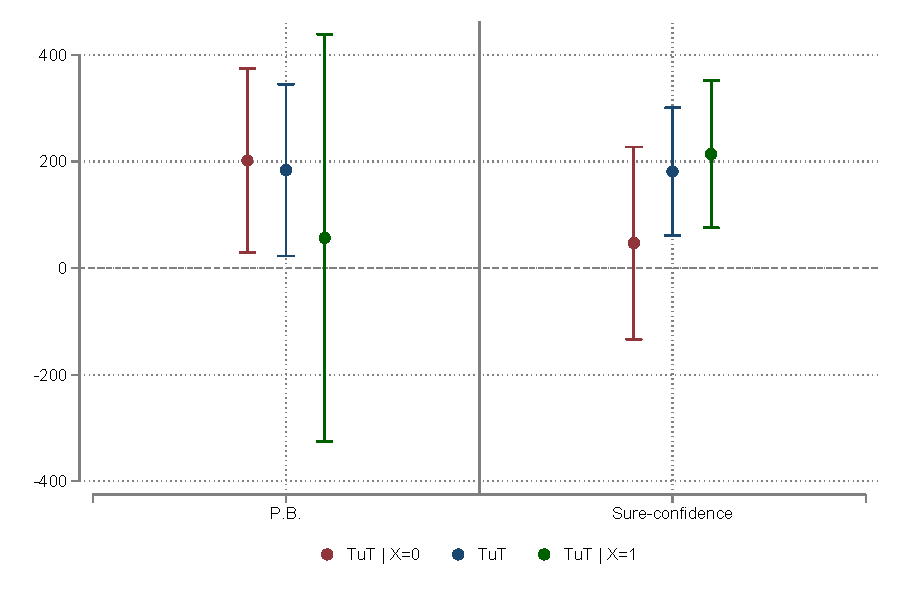
\includegraphics[width=0.65\textwidth]{Figuras/tut_beh_partition.pdf} 
    \end{center}  
 \footnotesize{Each panel in this figure shows how the estimated treatment on the untreated (TUT) effect varies with a binary survey variable $X_i$. In the left panel (P.B.), $X_i = 1$ if borrower $i$ is ``present-biased'' based on her responses to the time preference questions from our survey. In the right panel (Sure-confidence) $X_i = 1$ if  borrower $i$ reported that she was certain to recover her pawn, zero otherwise. }
    \label{tut_beh_partition}
      %\footnotesize{ \textit{Do file: }  \texttt{partition_tut.do}

\end{figure}
\subsection{Sure Confidence} \label{App_sureconfidence}

\begin{figure}[H]
\caption{Determinants sure confidence.}
    \begin{center}
    \begin{subfigure}{0.60\textwidth}
        \centering
        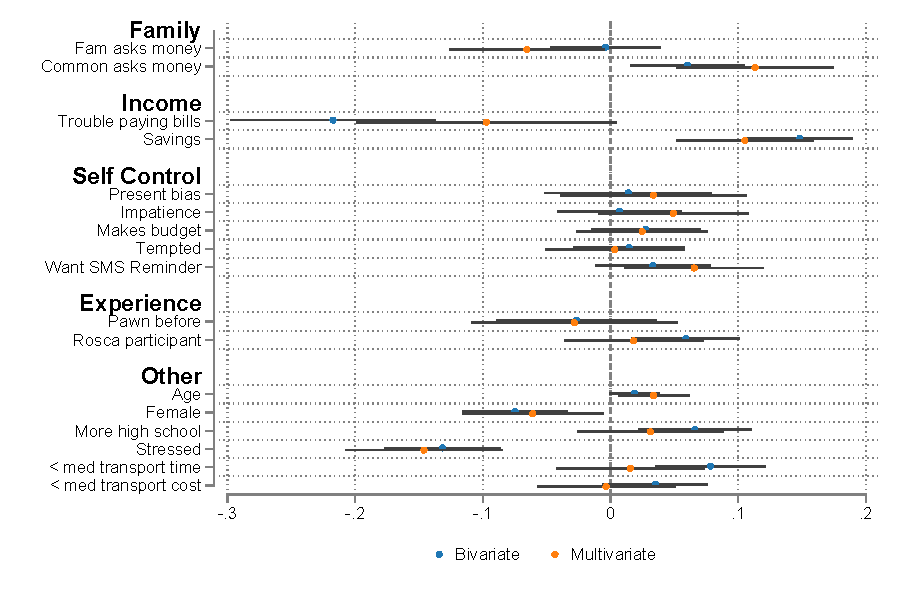
\includegraphics[width=\textwidth]{Figuras/determinants_confidence_100.pdf}
    \end{subfigure}
    \end{center}
     \footnotesize{The above figure shows the determinants in a bivariate and multivariate OLS regression of sure confidence among the non-choosers. Sure confidence is a binary variable defined to be one when people report a 100\% probability of recovery.}
    \label{determinants_sure}
%\textit{Do file: } \texttt{determinants_sure_confidence.do}       
\end{figure}


\newpage


%\section{ Heterogeneity and Bounds}
\section{Bounds, FOSD and Rank Invariance} \label{bounds_FOSD}

%\subsection{Testing for heterogeneity}
%\label{append:chernozhukov}
%If the treatment effects $Y_{i1} - Y_{i0}$ are constant across $i$, then we must have
%\[
%\text{ATE}(X_i) \equiv \mathbbm{E}[Y_{i1} - Y_{i0} |X_i] = \mathbbm{E}[Y_{i1} - Y_{i0}] \equiv \text{ATE}
%\]
%for any covariates $X_i$ that vary across $i$. If, on the other hand, $\text{ATE}(X_i)$ can be predicted using some scalar function $\tau(\cdot)$ of $X_i$, then the average treatment effect function is not constant so there must be treatment effect heterogeneity. 
%
%We operationalize this idea using a two-step approach proposed by \cite{chernozhukov2018generic}.  We begin by randomly dividing the participants in the forced arms of the experiment ($Z_i \neq 2$) into two groups: a training set and a test set.
%These sets are constructed to ensure that all observations from a given branch-day cluster are allocated to the same set.
%This avoids inferential problems that could arise from correlated unobservables within clusters.
%In the first step, we apply the generalized random forest approach of \cite{atheygrf} to the training set to estimate two proxy predictors: $\psi(\cdot|\text{Training})$ approximates the untreated potential outcome function, $\mathbbm{E}[Y_{i0}|X_i] = \mathbbm{E}[Y_i|Z_i=0,X_i]$, while  $\tau(\cdot|\text{Training})$, approximates the ATE function
%\[
%\text{ATE}(X_i) = \mathbbm{E}[Y_i|Z_i=1,X_i] - \mathbbm{E}[Y_i|Z_i=0, X_i].
%\]
%The proxy predictors need not be unbiased or even consistent estimators of the functions they aim to approximate: the goal of this exercise is merely to find a scalar function of $X_i$ that \emph{accurately predicts} $\text{ATE}(X_i)$.
%In the second step we fit a linear regression model to data from the training set using regressors constructed from the proxy functions $\psi(\cdot|\text{Training})$ and $\tau(\cdot|\text{Training})$ constructed in the first step. In particular, we estimate 
%\begin{equation}
%Y_i = \alpha_0 + \alpha_1 \psi_i + \beta_1 (Z_i - \mathbbm{E}[Z_i]) + \beta_2 (Z_i - \mathbbm{E}[Z_i])(\tau_i - \mathbbm{E}[\tau_i]) + \epsilon_i
%\label{eq:chernreg}
%\end{equation}
%where $\psi_i \equiv \psi(X_i|\text{Training})$ and $\tau_i \equiv \tau(X_i|\text{Training})$.\footnote{This is a slightly simpler regression than the one proposed in equation (3.1) of \cite{chernozhukov2018generic}, which involves propensity score weights. Because the random assignment of $Z$ in our experiment does \emph{not} condition on $X$, the propensity score weights in our case are constant over $X$ and hence drop out.} As shown by \cite{chernozhukov2018generic}, the coefficients $\beta_1$ and $\beta_2$ from \eqref{eq:chernreg} identify the \emph{best linear predictor} of the conditional ATE based on $\tau(\cdot|\text{Training})$, namely
%\[
%\beta_1 = \mathbbm{E}[\text{ATE}(X_i)] = \text{ATE}, \quad
%\beta_2 = \frac{\text{Cov}[\text{ATE}(X_i), \tau_i]}{\text{Var}(\tau_i)}.
%\]
%If treatment effects are homogeneous we must have $\beta_2 = 0$. Rejecting this hypothesis establishes that $\tau_i$ predicts $\text{ATE}(X_i)$ and hence that $\Delta_i$ varies. 
%Since $\tau_i$ and $\psi_i$ do not depend on the test set, inference for the regression in \eqref{eq:chernreg} is straightforward conditional on the Training/Test split.  
%Our estimate for $\beta_2$ is 2.56 with a one-sided heteroskedasticity-robust (HC3) standard error of 0.43.
%Thus we easily reject the null hypothesis of homogeneous treatment effects.

%\todo[inline]{Discuss the results here.}

%\todo[inline]{Issac: re-run this exercise with removing the propensity score weights $p(Z)$. Presumably it shouldn't change anything, but it's simpler to explain what we do and probably less noisy}

%\begin{table}[H]
%\begin{center}
%\footnotesize{% Table generated by Excel2LaTeX from sheet 'test_calibration_2'
\begin{tabular}{rccccc}
\toprule
      & \multicolumn{5}{c}{Test Calibration} \\
\midrule
      & \multicolumn{2}{c}{With PS} &       & \multicolumn{2}{c}{Without PS} \\
\cmidrule{2-3}\cmidrule{5-6}      & \multicolumn{2}{c}{APR} &       & \multicolumn{2}{c}{APR} \\
\cmidrule{2-3}\cmidrule{5-6}      & BVC   & BVC + survey variables &       & BVC   & BVC + survey variables \\
\midrule
      & (1)   & (2)   &       & (3)   & (4) \\
\midrule
\midrule
\multicolumn{1}{l}{Mean Forest Prediction} & 0.9797 & 0.9983 &       & 0.8302 & 0.8816 \\
      & (0.1335) & (0.1165) &       & (0.1198) & (0.1034) \\
\multicolumn{1}{l}{Differential Forest Prediction} & 0.9486 & 1.3224 &       & 0.8107 & 1.2027 \\
      & (0.1270) & (0.2073) &       & (0.1163) & (0.1861) \\
\bottomrule
\bottomrule
\end{tabular}%
}
%\end{center}
%\end{table}

%\todo[inline]{Some Questions for Issac: (1) How are we carrying out the sample splitting? If we cluster standard errors at the branch-day level, we should take this into account when we split. (2) How are you carrying out inference for $\beta_2$? Chernozhukov et al discuss two approaches: ``conditional'' and ``variational.'' The former is simpler as it conditions on the training/test split. The latter is a bit more involved, since one accounts for uncertainty arising from different splits. (3) What are the details of the random forest procedure employed here? (Tuning parameters choice, etc.) We should put them into the appendix.}

%\newpage

\begin{figure}[!h]
   \caption{Fan \& Park bounds for benefit in APR\%.}
    \begin{center}
    \begin{subfigure}{0.65\textwidth}
        \caption{APR Bounds}
        \centering
        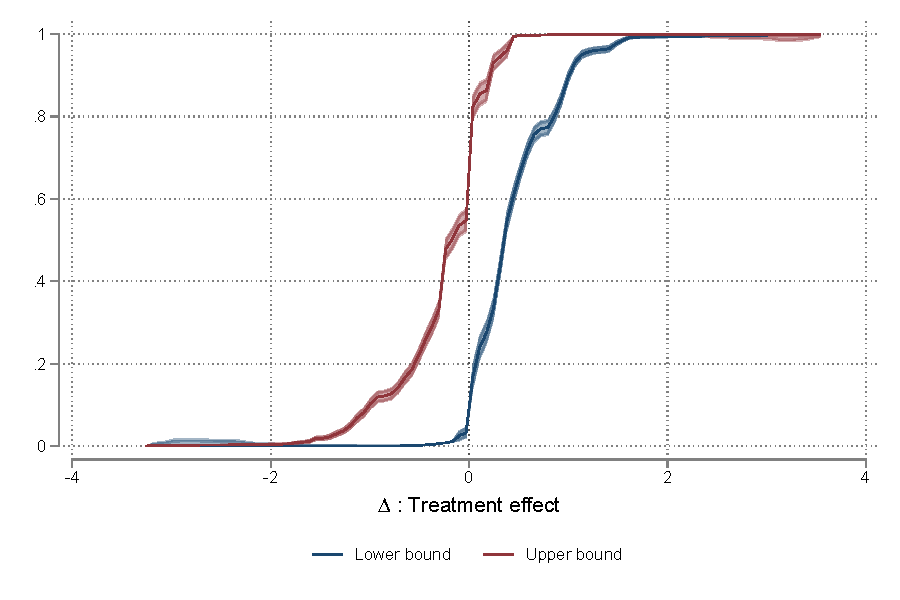
\includegraphics[width=\textwidth]{Figuras/fan_park_bounds_apr.pdf}
    \end{subfigure}
    \end{center}
          \footnotesize{This figure depicts the \cite{fan2010sharp} bounds on the distribution $F_\Delta$ of individual treatment effects $\Delta \equiv (Y_1 - Y_0)$, described in Section \ref{sec:bounds}, for the APR outcome.
    The dark red curve and light red shaded region give the estimated upper bound function $\overline{F}$ for $F_\Delta$ and associated (pointwise) 95\% confidence interval. 
    The dark blue curve and light blue shaded region give the estimated lower bound function $\underline{F}$ for $F_\Delta$ and associated (pointwise) 95\% confidence interval.
    Confidence intervals are computed using the asymptotic distribution for the bounds.  Evaluating the bounds at $\delta = 0$, we see that between 23\% and 97\% of borrowers have a positive individual treatment effect.}
     \label{fan_park_bounds}
%\textit{Do file: } \texttt{fan\_park\_bnds.do}       
\end{figure}

\begin{figure}[!h]
\caption{Distribution of treatment effects under rank invariance.}        
    \begin{center}
       \begin{subfigure}{0.49\textwidth}
        \caption{APR benefit}
        \centering
        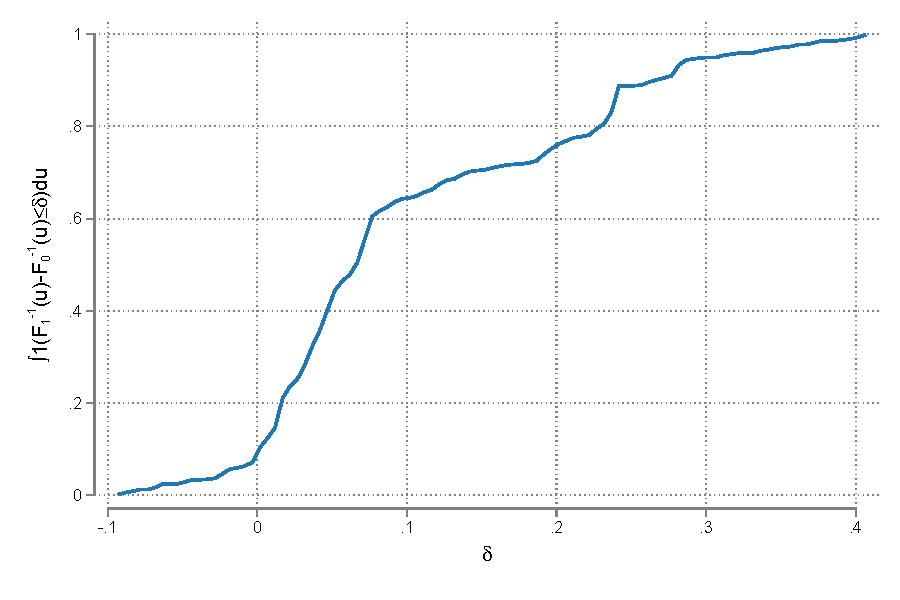
\includegraphics[width=\textwidth]{Figuras/te_rankinvariance_apr.pdf}
    \end{subfigure} 
   \begin{subfigure}{0.49\textwidth}
        \caption{Financial benefit}
        \centering
        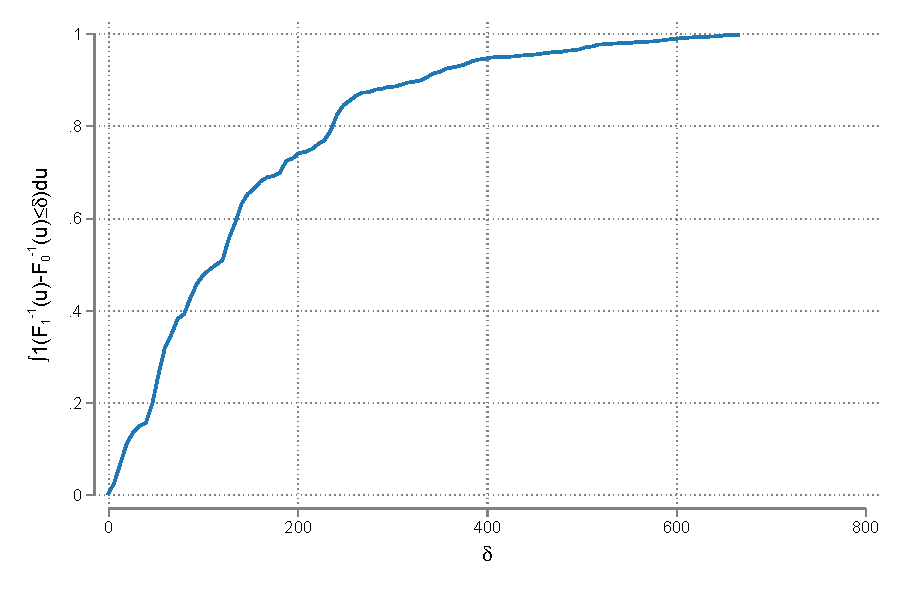
\includegraphics[width=\textwidth]{Figuras/te_rankinvariance_fc_admin.pdf}
    \end{subfigure} 
    \end{center}
    \footnotesize{This figure shows the CDF of individual treatment effects under the assumption of rank invariance, computed from $F_\Delta(\delta) = \int_0^1 \mathbbm{1}\{ F_1^{-1}(u) - F_0^{-1}(u)\leq \delta\}\,\mathrm{d}u$ where $F_1^{-1}$ and $F_0^{-1}$ are the quantile functions of $Y_1$ and $Y_0$.}
\label{te_rankinvariance}
    %The dotted line at the bottom of panels (a) and (b)   the empirical cumulative distribution function APR and financial cost of financial cost. It does this separately for the fee-forcing contract and for the status-quo contract. The dotted line at the bottom is the difference of the control CDF minus the forced CDF arm. It shows that the CDF of the status quo contract is always below that of the fee-forcing (and this difference is significant for the points indicated by the blue line).
    % \texttt{te_rankinvariance.do}}
\end{figure}


\newpage 

\section{ Causal Random Forest, CATE, and `mistakes'}\label{app:cate}


To estimate conditional average treatment effects given administrative and survey data, we use the function \texttt{causal\_forest()} of the \texttt{grf} R package; to estimate conditional TOT and TUT effects we use the \texttt{instrumental\_forest()} function from the same package.
In each case, we use the default parameter values from the \texttt{grf} package with one exception: we increase the number of trees from the default value of 2000 to 5000.
The functions \texttt{causal\_forest()} and \texttt{instrumental\_forest()} implement special cases of the ``generalized random forest'' methods of \cite{atheygrf}.
In broad strokes, these functions combine a large number of regression trees that recursively partition the covariate space to estimate conditional average effects.
% Figure \ref{causal_tree1} illustrates the partition that emerges from one of the trees in our causal forest implementation.
The trees are ``honest'' in that observations used to determine the optimal partition are not used to estimate effects, and vice-versa.
While closely related to more familiar ``regression-tree'' random forests, the generalized random forest approach explicitly targets the parameter of interest--a conditional ATE or IV estimand--when choosing the optimal covariate partition.
\footnote{For more details, see \cite{atheygrf} and the \texttt{grf} documentation: \url{https://grf-labs.github.io/grf/}. When constructing our random forest estimates of heterogeneous treatment effects, we use observations for all borrowers who answered at least \emph{part} of the intake survey.
We impute the median response for the missing values, while also including an indicator whether the variable originally had a missing value. Results are similar if we manually include interactions between the original/imputed variable and an indicator for missingness. This is as expected, given that tree-based methods by their nature ``automatically'' consider interactions of arbitrary orders.}

\begin{figure}[!h]
     \caption{Heterogeneous Treatment Effects.} 
     \label{heterogeneous_effects}    
    \begin{center}
     \begin{subfigure}{0.35\textwidth}
       \centering
      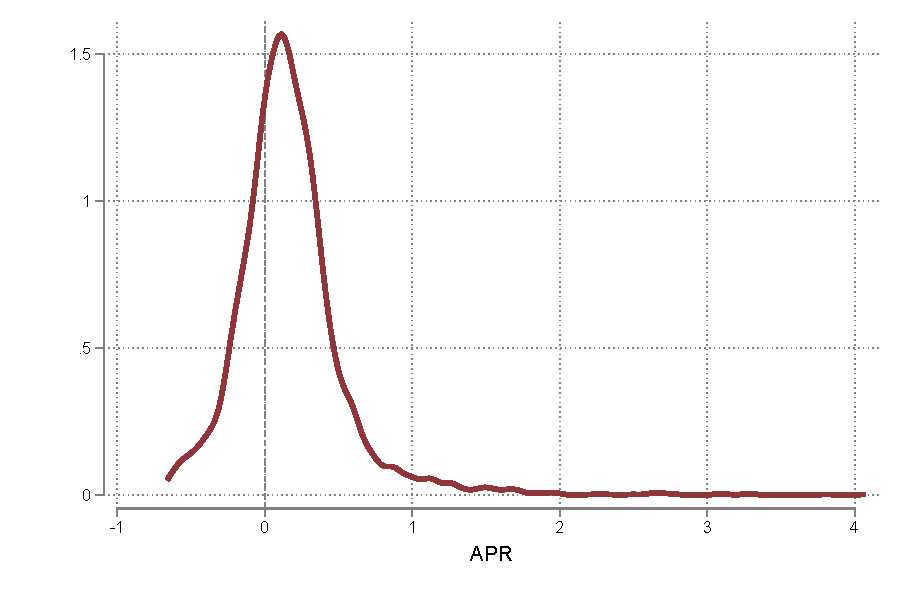
\includegraphics[width=\textwidth]{Figuras/he_dist_tau_hat_tot.pdf}
          \caption{ToT}
    \end{subfigure}
    \begin{subfigure}{0.35\textwidth}
       \centering
      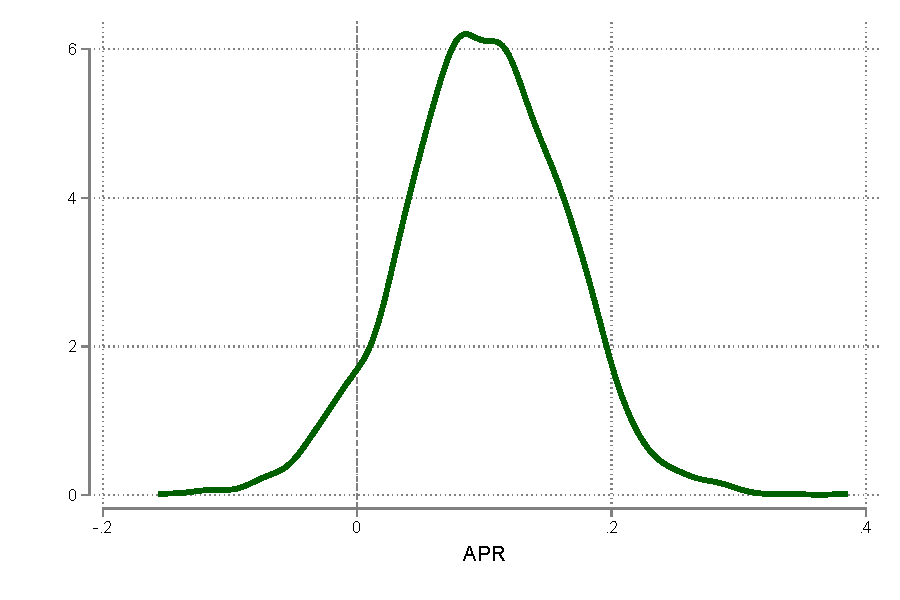
\includegraphics[width=\textwidth]{Figuras/he_dist_tau_hat_tut.pdf}
          \caption{TuT}
    \end{subfigure} 
       \begin{subfigure}{.35\textwidth}
        \centering
        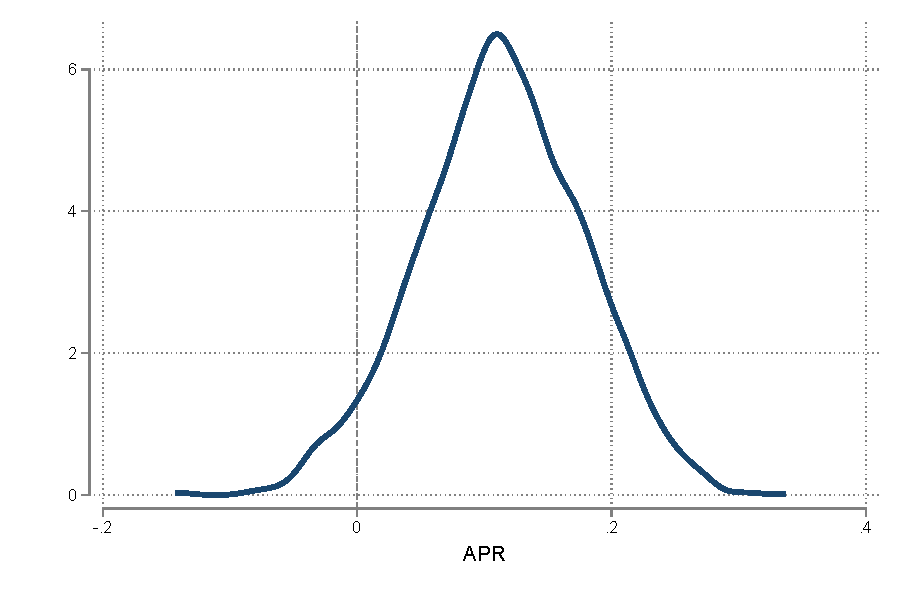
\includegraphics[width=\textwidth]{Figuras/he_dist_tau_hat_eff.pdf}
        \caption{ATE}
    \end{subfigure} 
    \end{center}
  %\footnotesize{ } \textit{Do file: }  \texttt{cate_dist.do}
\end{figure}

\begin{figure}[h!]
   \caption{Conditional ATEs from ``wide'' and ``narrow'' covariate sets.}
    \begin{center}
    \begin{subfigure}{0.75\textwidth}
        \centering
        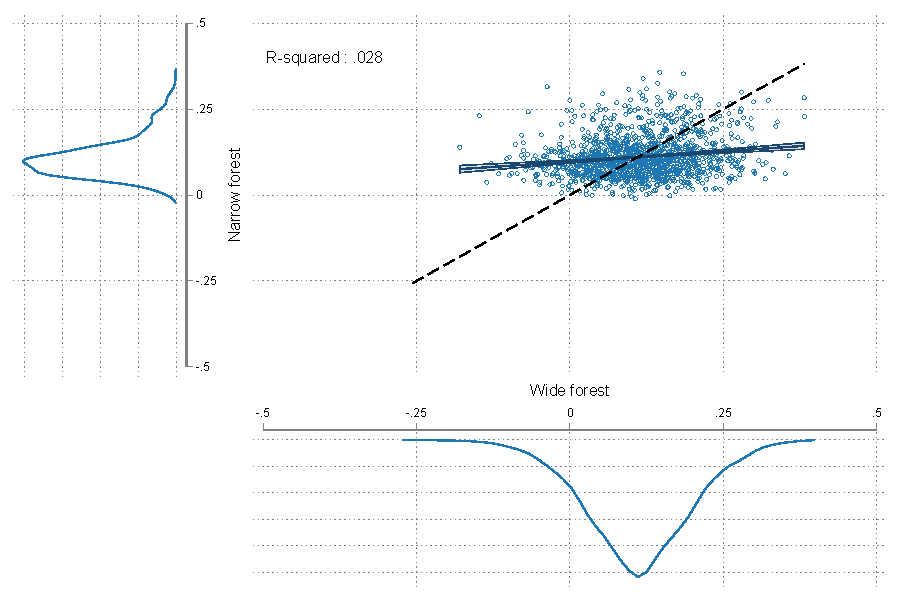
\includegraphics[width=\textwidth]{Figuras/scatter_hist_wide_narrow.pdf}
    \end{subfigure}
    \end{center}
        \footnotesize{This figure plots the relationship between the causal forest conditional ATE estimates from Section \ref{sec:RF} that use the ``wide'' set of covariates (all intake survey responses) and those based on a restricted ``narrow'' set of covariates (age, gender, HS education, and previous borrowing). The scatterplot graphs one estimate versus the other, with the ``wide'' covariate set on the horizontal axis and the ``narrow'' set on the vertical axis. The density plots on each axis show the estimated marginal distribution of conditional ATEs under each covariate set. The density for the ``wide'' covariate set is considerably more dispersed, as the causal forest based on this set of covariates captures considerably more treatment effect heterogeneity.}
    \label{wide_narrow_forests}

%\textit{Do file: } \texttt{wide_narrow_forests.do}       
\end{figure}

\newpage 

\section{Testable Implications of the Exclusion Restriction} \label{sec:testing_exclusion}

%This section describes the testable implications of our exclusion restrictions: \eqref{eq:exclusion0} and \eqref{eq:exclusion1} from Section \ref{sec:potentialOutcomes}. 
%To consider possible violations of these conditions, we require some additional notation.
As above, let $Y_0 \equiv Y(d=0,z=0)$ and $Y_1 \equiv Y(d=1,z=1)$ denote the potential outcomes under \emph{forced treatment}: $Y_0$ is the potential outcome when forced into the status quo contract and $Y_1$ when forced into the commitment contract. 
Further let $Y_{0,2} \equiv Y(d=0,z=2)$ and $Y_{1,2} \equiv Y(d=1,z=2)$ denote the potential outcomes under \emph{free choice of treatment}: $Y_{0,2}$ is the potential outcome when choosing the status quo contract and $Y_{1,2}$ when choosing the commitment contract. 
Using this notation, \eqref{eq:exclusion0} becomes $Y_0 = Y_{0,2}$ and while \eqref{eq:exclusion1} becomes $Y_1 = Y_{1,2}$.
Without imposing these, Assumption \ref{assump:randchoice}(iii) becomes 
\[
Y = \mathbbm{1}(Z =0) Y_{0} + \mathbbm{1}(Z = 1)  Y_{1}  + \mathbbm{1}(Z = 2) \left[(1 - C) Y_{0,2} + C Y_{1,2} \right]
\]
but parts (i) and (ii) continue to hold.
Accordingly, parts (i)--(iii) of Lemma \ref{lem_randchoice} are unchanged, while parts (iv) and (v) become
\[
\mathbbm{E}(Y|D=0,Z=2) = \mathbbm{E}(Y_{0,2}|C=0), \quad
\mathbbm{E}(Y|D=1,Z=2) = \mathbbm{E}(Y_{0,1}|C=1).
\]
Using these expressions, the testable restrictions we consider here are as follows:
\begin{align}
\label{eq:exclusion_append0}
\mathbbm{E}(Y_0|C=0) &= \mathbbm{E}(Y_{0,2}|C=0) \\
\label{eq:exclusion_append1}
\mathbbm{E}(Y_1|C=1) &= \mathbbm{E}(Y_{1,2}|C=1).
\end{align}
%Equation \ref{eq:exclusion_append0} is a restriction on the average potential outcomes of non-choosers that we use to point identify the TUT effect.
%It says that someone who \emph{would} choose the control condition when given a choice, experiences the same potential outcome, on average, when \emph{assigned} to the control condition.
%Equation \ref{eq:exclusion_append1} is a restriction on the average potential outcomes of choosers that we use to point identify the TOT effect.
%It says that someone who \emph{would} choose the commitment contract when given a choice, experiences the same potential outcome, on average, when \emph{assigned} to this condition.
Because they refer to different groups of people--choosers versus non-choosers--either of \eqref{eq:exclusion_append0}  and \eqref{eq:exclusion_append1} could hold when the other is violated.
For this reason we consider each in turn.
Our approach is closely related to arguments from \cite{huber_mellace} and \cite{BinaryRegressor}, among others.
%As such, the following is a heuristic explanation rather than a fully-rigorous proof.
%See the aforementioned papers for more details of how to make this argument fully rigorous.

Consider first \eqref{eq:exclusion_append0}.
Let $p \equiv \mathbbm{P}(C=1) = \mathbbm{P}(D=1|Z=2)$ denote the share of choosers in the population.
This value is point identified regardless of whether the exclusion restriction holds.
Because $Z$ was randomly assigned, a fraction $p$ of borrowers with $Z=0$ are choosers while the remaining $(1-p)$ are non-choosers.
It follows that, regardless of whether the exclusion restriction holds, the observed distribution of $Y|Z=0$ is a mixture of $Y_0|C=0$ and $Y_0|C=1$ with mixing weights $(1-p)$ and $p$.
This allows us to construct a pair of bounds for $\mathbb{E}(Y_0|C=0)$ as follows.
The non-choosers must lie \emph{somewhere} in the distribution of $Y|Z=0$.
Consider the two most extreme possibilities: they could occupy the bottom $(1-p)\times 100\%$ of the distribution or the top $(1-p)\times 100\%$ of the distribution.
For this reason, computing the average of the \emph{truncated} distribution of $Y|Z=0$, cutting out the top $p\times 100\%$, provides a lower bound for the average of $Y_0$ among non-choosers.
Similarly, cutting out the bottom $p \times 100\%$ provides an upper bound.
Let $y^0_{1-p}$ denote the $(1-p)$ quantile of $Y|Z=0$ and $y^0_{p}$ denote the $p$ quantile of the same distribution.
Using this notation, the bounds are given by
\[
\mathbb{E}\left(Y|Z=0, Y\leq y^0_{1-p}\right)\leq \mathbb{E}(Y_0|C=0) \leq \mathbb{E}\left(Y|Z=0, Y \geq y^0_p\right) 
\]
These bounds do not rely on the exclusion restriction.
Under Equation \ref{eq:exclusion_append0}, however, we know that $\mathbb{E}(Y_0|C=0)=\mathbb{E}(Y|D=0,Z=2)$.
Therefore, if the exclusion restriction for non-choosers holds, we must have
\begin{equation}
\mathbb{E}\left(Y|Z=0, Y\leq y^0_{1-p}\right)\leq \mathbb{E}(Y|D=0,Z=2) \leq \mathbb{E}\left(Y|Z=0, Y \geq y^0_p\right).
\label{eq:testable0}
\end{equation}
Equation \ref{eq:testable0} provides a pair of testable implications of \eqref{eq:exclusion_append0}.
If either inequality is violated, then the exclusion restriction for non-choosers fails.
In our experiment, $\widehat{p} = \widehat{\mathbbm{P}}(D=1|Z=2) = 0.11$. For the APR outcome we estimate
\[
\widehat{\mathbbm{E}}(Y_\text{APR}|Z=0,Y_\text{APR}\leq y^0_{0.89}) = 0.48, \quad
\widehat{\mathbbm{E}}(Y_\text{APR}|Z=0, Y_\text{APR}\geq y^0_{0.11}) = 0.62.
\]
Since $\widehat{\mathbbm{E}}(Y_\text{APR}|D=0,Z=2) = 0.58$ falls between these bounds, we find no evidence against the exclusion restriction for non-choosers. 
The same result holds for the financial cost outcome: results available upon request. 
%Repeating this exercise for the financial cost outcome, we see that $\widehat{\mathbbm{E}}(Y_\text{FC}|D=0,Z=2) = 973$ likewise falls between 
%\[
%\widehat{\mathbbm{E}}(Y_\text{FC}|Z=0,Y_\text{FC}\leq y^0_{0.89}) = 626, \quad
%\widehat{\mathbbm{E}}(Y_\text{FC}|Z=0, Y_\text{FC}\geq y^0_{0.11}) = 1046 
%\]
%so we again find no evidence against the exclusion restriction for non-choosers.

We can use an analogous approach to construct testable implications for \ref{eq:exclusion_append1}, yielding 
%Because $Z$ was randomly assigned, a fraction $p$ of participants with $Z = 1$ are choosers so the distribution of $Y|Z=1$ is a mixture of $Y_1|C=1$ and $Y_1|C=0$ with mixing weights $p$ and $1 -p$.
%The participants with $C = 1$ must lie \emph{somewhere} in the distribution of $Y_0|Z=1$ so again consider the two most extreme cases: they could occupy the bottom or the top $p\times 100\%$ of the distribution. 
%\[
%\mathbbm{E}\left(Y|Z=1,Y\leq y^1_{p}\right) \leq \mathbbm{E}(Y_1|C=1) \leq \mathbbm{E}\left(Y|Z=1,Y \geq y^1_{1-p}\right)
%\]
%As above, these bounds do not rely on the exclusion restriction.
%If Equation \ref{eq:exclusion_append1} holds, however, we know that $\mathbb{E}(Y|D=1,Z=2) = \mathbb{E}(Y_1|C=1)$, yielding the following testable implications for choosers
\begin{equation}
\mathbbm{E}\left(Y|Z=1,Y\leq y^1_{p}\right) \leq \mathbbm{E}(Y|D=1,Z=2) \leq \mathbbm{E}\left(Y|Z=1,Y \geq y^1_{1-p}\right).
\label{eq:testable1}
\end{equation}
where $y^1_p$ and $y^1_{1-p}$ are the $p$ and $1 - p$ quantiles of the distribution of $Y|Z=1$.
If either inequality is violated, then the exclusion restriction from Equation \ref{eq:exclusion_append1} fails.
Again, in our experiment $\widehat{p}=0.11$. For the APR outcome we estimate
\[
\widehat{\mathbbm{E}}(Y|Z=1,Y\leq y^1_{0.11}) = 0.06, \quad
\widehat{\mathbbm{E}}(Y|Z=1,Y\geq y^1_{0.89}) = 1.28
\]
Since $\widehat{\mathbbm{E}}(Y_\text{APR}|D=1,Z=2) = 0.43$ falls between these bounds, we find no evidence against the exclusion restriction for the choosers. 
The same holds for the financial cost outcome: results available upon request.
%Repeating this exercise for the financial cost outcome, we see  that $\widehat{\mathbbm{E}}(Y_\text{FC}|D=1,Z=2)= 570$ likewise falls between
%\[
%\widehat{\mathbbm{E}}(Y|Z=1,Y\leq y^1_{0.11}) = 53, \quad
%\widehat{\mathbbm{E}}(Y|Z=1,Y\geq y^1_{0.89}) = 2934
%\]
%so we again find no evidence against the exclusion restriction for the choosers.

%The aforementioned bounds for $\mathbbm{E}(Y_0|C=0)$ and $\mathbbm{E}(Y_1|C=1)$ can alternatively be used construct partial identification bounds for the TOT and TUT effects that do not rely on our exclusion restrictions. If the TOT or TUT expressions from \eqref{eq:TOT} and \eqref{eq:TUT} fall \emph{outside} the partial identification bounds, this is equivalent to finding a violation of \ref{eq:testable0} or \ref{eq:testable1}. We implement these bounds for the TOT and TUT in our companion STATA package.


\section{Estimation and Inference} 
\label{sec:estimation_inference}

\subsection{Regression-based Estimation of TOT, TUT, ASG, ASL, and ASB}

Let $Z_0 \equiv \mathbbm{1}\{Z=0\}$, $Z_1 \equiv \mathbbm{1}\{Z=1\}$, and $Z_2 \equiv \mathbbm{1}\{Z=2\}$.
Under standard regularity conditions, the following proposition shows that an IV regression of $Y$ on an intercept, $Z_1$ and $Z_2 D$ with instruments $(1, Z_0, Z_1)$ provides consistent estimates the ATE and TOT, while an IV regression of $Y$ on an intercept, $-Z_0$ and $-Z_2(1-D)$ with the same instrument set consistently estimates the ATE and TUT effects.

\begin{prop} 
\label{prop:TOTandTUTregs}
Under Assumption \ref{assump:randchoice}, 
\begin{enumerate}[(i)] 
\item $Y = \mathbbm{E}(Y_0) + \text{ATE}\times Z_1 + \text{TOT} \times Z_2 D + U$
\item $Y = \mathbbm{E}(Y_1) + \text{ATE}\times -Z_0 + \text{TUT} \times -Z_2 (1 - D) + V$
\end{enumerate}
where $\mathbbm{E}(U|Z) = \mathbbm{E}(V|Z) = 0$.
\end{prop}

\begin{proof}[Proof of Proposition \ref{prop:TOTandTUTregs}]
For part (i), since $Z_2 D = Z_2 C$ and $(Z_0 + Z_1 + Z_2) = 1$, Assumption \ref{assump:randchoice} (iii) implies $Y= Y_0 + Z_1 (Y_1 - Y_0) + Z_2D(Y_1 - Y_0)$.
Now define 
\[
U \equiv [Y_0 - \mathbbm{E}(Y_0)] + Z_1[(Y_1 - Y_0) - \text{ATE}] + Z_2 D[(Y_1 - Y_0) - \text{TOT}].
\]
Since $Z_2 D = Z_2 C$ and $Z$ is independent of $(Y_1, Y_0)$ by Assumption \ref{assump:randchoice} (i), it follows that $\mathbbm{E}(U|Z) = Z_2 \mathbbm{E}\left[C\left\{(Y_1 - Y_0) - \text{TOT}\right\}|Z\right]$.
Thus, by iterated expectations,
\begin{align*}
\mathbbm{E}\left[C\left\{(Y_1 - Y_0) - \text{TOT}\right\}|Z\right] 
%&=  \mathbbm{P}(C=1|Z) \left[\mathbbm{E}(Y_1 - Y_0|C=1,Z)  - \text{TOT}\right]\\
&= \mathbbm{P}(C=1)\left[\mathbbm{E}(Y_1 - Y_0|C=1) - \text{TOT} \right]=0
\end{align*}
since $Z$ is independent of $(Y_0, Y_1)$ given $C$, an implication of Assumption \ref{assump:randchoice} (i).

For part (ii), since $Z_2(1 - C)= Z_2(1 - D)$ and $(Z_1 + Z_2) = 1 - Z_0$,  Assumption \ref{assump:randchoice} (iii) implies $Y= Y_1 - Z_0 (Y_1 - Y_0) - Z_2(1 - D) (Y_1 - Y_0)$.
Define 
\[
V \equiv [Y_1 - \mathbb{E}(Y_1)] - Z_0[(Y_1 - Y_0) - \text{ATE}] - Z_2(1 - D)[(Y_1 - Y_0) - \text{TUT}].
\]
Since $Z_2(1 - D) = Z_2 (1 - C)$ and $Z$ is independent of $(Y_0, Y_1)$ by Assumption \ref{assump:randchoice} (i),
$\mathbb{E}(V|Z) = -Z_2\mathbb{E}[(1 - C)\left\{(Y_1 - Y_0) - \text{TUT}\right\}|Z]$.
Thus, by iterated expectations,
\begin{align*}
\mathbb{E}[(1 - C)\left\{(Y_1 - Y_0) - \text{TUT}\right\}|Z]
%&= \mathbb{P}(C=0|Z)\left[ \mathbb{E}(Y_1 - Y_0|C=0, Z) - \text{TUT}\right]\\
&= \mathbb{P}(C=0|Z) \left[ \mathbb{E}(Y_1 - Y_0|C=0) - \text{TUT}\right] = 0
\end{align*}
since $Z$ is independent of $(Y_0, Y_1)$ given $C$, an implication of Assumption \ref{assump:randchoice} (i).
\end{proof}

%\begin{prop} 
%\label{prop:TOTreg}
%Under Assumption \ref{assump:randchoice}, $Y = \mathbbm{E}(Y_0) + \text{ATE}\times Z_1 + \text{TOT} \times Z_2 D + U$ where $\mathbbm{E}(U|Z) = 0$.
%\end{prop}
%
%\begin{proof}
%By Assumption \ref{assump:randchoice} (iii),
%$Y= Y_0 + Z_1 (Y_1 - Y_0) + Z_2D(Y_1 - Y_0)$
%%\begin{align*}
%%Y &= Z_0 Y_0 + Z_1 Y_1 + Z_2[(1 - C) Y_0 + CY_1] 
%%= (Z_0 + Z_2)Y_0 + Z_1 Y_1 + Z_2C(Y_1 - Y_0)\\
%%&= (Z_0 + Z_1 + Z_2)Y_0 + Z_1 (Y_1 - Y_0) + Z_2D(Y_1 - Y_0) 
%%= Y_0 + Z_1 (Y_1 - Y_0) + Z_2D(Y_1 - Y_0).
%%\end{align*}
%because $Z_2 D = Z_2 C$ and $(Z_0 + Z_1 + Z_2) = 1$.
%Thus, defining 
%\[
%U \equiv [Y_0 - \mathbbm{E}(Y_0)] + Z_1[(Y_1 - Y_0) - \text{ATE}] + Z_2 D[(Y_1 - Y_0) - \text{TOT}]
%\]
%by construction we have $Y = \mathbbm{E}(Y_0) + \text{ATE} \times Z_1 + \text{TOT} \times Z_2 D+ U$.
%Since $Z_2 D = Z_2 C$ and $Z$ is independent of $(Y_1, Y_0)$ by Assumption \ref{assump:randchoice} (i), we have
%\begin{align*}
%\mathbbm{E}(U|Z) 
%%&= [\mathbbm{E}(Y_0|Z) - \mathbbm{E}(Y_0)]  + Z_1[\mathbbm{E}(Y_1 - Y_0|Z) - \text{ATE}] +  \mathbbm{E}\left[Z_2 D\left\{(Y_1 - Y_0) - \text{TOT}\right\}|Z\right]\\
%%&= [\mathbbm{E}(Y_0) - \mathbbm{E}(Y_0)]  + Z_1[\mathbbm{E}(Y_1 - Y_0) - \text{ATE}] + Z_2 \mathbbm{E}\left[C\left\{(Y_1 - Y_0) - \text{TOT}\right\}|Z\right]\\
%&= Z_2 \mathbbm{E}\left[C\left\{(Y_1 - Y_0) - \text{TOT}\right\}|Z\right].
%\end{align*}
%Finally, by iterated expectations
%\begin{align*}
%\mathbbm{E}\left[C\left\{(Y_1 - Y_0) - \text{TOT}\right\}|Z\right] 
%%&=  \mathbbm{P}(C=1|Z) \left[\mathbbm{E}(Y_1 - Y_0|C=1,Z)  - \text{TOT}\right]\\
%&= \mathbbm{P}(C=1)\left[\mathbbm{E}(Y_1 - Y_0|C=1) - \text{TOT} \right]=0
%\end{align*}
%since $Z$ is conditionally independent of $(Y_0, Y_1)$ given $C$, an implication of \ref{assump:randchoice} (i).
%\end{proof}
%
%%The next proposition provides regression-based estimates of the ATE and TUT.
%\begin{prop}
%\label{prop:TUTreg}
%Under Assumption \ref{assump:randchoice}, $Y = \mathbbm{E}(Y_1) + \text{ATE}\times -Z_0 + \text{TUT} \times -Z_2 (1 - D) + V$ where $\mathbb{E}(V|Z) = 0$.
%Thus, an IV regression of $Y$ on an intercept, $-Z_0$ and $-Z_2(1-D)$ with instruments $(1, Z_0, Z_1)$ provides consistent estimates of the ATE and TUT effects.
%\end{prop}
%
%\begin{proof}
%By Assumption \ref{assump:randchoice} (iii),
%$Y= Y_1 - Z_0 (Y_1 - Y_0) - Z_2(1 - D) (Y_1 - Y_0)$
%%\begin{align*}
%%Y %&= Z_0 Y_0 + Z_1 Y_1 + Z_2[(1 - C) Y_0 + CY_1] 
%%&= Z_0 Y_0 + Z_1 Y_1 + Z_2[(1 - C) (Y_0 - Y_1) + Y_1]
%%&= Z_0 Y_0 + (Z_1 + Z_2) Y_1 + Z_2(1 - C) (Y_0 - Y_1) = Z_0 Y_0 + (1 - Z_0) Y_1 + Z_2(1 - D) (Y_0 - Y_1) \\
%%= Y_1 - Z_0 (Y_1 - Y_0) - Z_2(1 - D) (Y_1 - Y_0)
%%\end{align*}
%since $Z_2(1 - C)= Z_2(1 - D)$ and $(Z_1 + Z_2) = 1 - Z_0$.
%Thus, defining 
%\[
%V \equiv [Y_1 - \mathbb{E}(Y_1)] - Z_0[(Y_1 - Y_0) - \text{ATE}] - Z_2(1 - D)[(Y_1 - Y_0) - \text{TUT}]
%\]
%by construction we have $Y = \mathbb{E}(Y_1) + \text{ATE} \times -Z_0 + \text{TUT} \times -Z_2(1 - D) + V$.
%Now, since $Z_2(1 - D) = Z_2 (1 - C)$ and $Z$ is independent of $(Y_0, Y_1)$ by Assumption \ref{assump:randchoice} (i),
%\begin{align*}
%\mathbb{E}(V|Z) 
%%&= [\mathbb{E}(Y_1|Z) - \mathbb{E}(Y_1)] - Z_0[\mathbb{E}(Y_1 - Y_0|Z) - \text{ATE}] - \mathbb{E}[Z_2(1 - D)\left\{(Y_1 - Y_0) - \text{TUT}\right\}|Z]\\
%%&= [\mathbb{E}(Y_1) - \mathbb{E}(Y_1)] - Z_0[\mathbb{E}(Y_1 - Y_0) - \text{ATE}] - Z_2\mathbb{E}[(1 - C)\left\{(Y_1 - Y_0) - \text{TUT}\right\}|Z]\\
%&= -Z_2\mathbb{E}[(1 - C)\left\{(Y_1 - Y_0) - \text{TUT}\right\}|Z].
%\end{align*}
%Finally, by iterated expectations,
%\begin{align*}
%\mathbb{E}[(1 - C)\left\{(Y_1 - Y_0) - \text{TUT}\right\}|Z]
%%&= \mathbb{P}(C=0|Z)\left[ \mathbb{E}(Y_1 - Y_0|C=0, Z) - \text{TUT}\right]\\
%&= \mathbb{P}(C=0|Z) \left[ \mathbb{E}(Y_1 - Y_0|C=0) - \text{TUT}\right] = 0
%\end{align*}
%since $Z$ is independent of $(Y_0, Y_1)$ given $C$, an implication of Assumption \ref{assump:randchoice} (i).
%\end{proof}

Since $\text{ASG} = \text{TOT} - \text{TUT}$, the preceding proposition provides a consistent estimate of the $\text{ASG}$ effect.
The $\text{ASB}$ effect, $\mathbbm{E}(Y_0|C=1) - \mathbb{E}(Y_0|C=0)$, can likewise be estimated by taking the difference of coefficients across two linear IV regressions with \emph{no intercept} and instrument sets $(Z_0, Z_2)$, as shown in the following proposition.

\begin{prop}
\label{prop:ASBreg}
Under Assumption \ref{assump:randchoice}
\begin{enumerate}[(i)]
    \item $(1 - D) Y = \mathbbm{E}(Y_{0}) \times Z_0 + \mathbbm{E}(Y_{0}|C=0) \times (1 - D)Z_2 + U_{0}$
    \item  $(1 - D) Y = \mathbbm{E}(Y_{0}) \times(Z_0 + Z_2) + \mathbbm{E}(Y_{0}|C=1)\times -DZ_2 + U_{1}$
\end{enumerate}
where $\mathbbm{E}(U_0|Z) = \mathbbm{E}(U_1|Z) = 0$.
%Thus, an IV regression of $(1 - D)Y$ on $Z_0$ and $(1 - D)Z_2$ with instruments $(Z_0, Z_2)$ and no intercept consistently estimates $\mathbb{E}(Y_0)$ and $\mathbb{E}(Y_0|C=0)$. 
%Similarly, an IV regression of $(1 - D)Y$ on $(Z_0 + Z_2)$ and $-DZ_2$ with instruments $(Z_0, Z_2)$ and no intercept consistently estimates $\mathbb{E}(Y_0)$ and $\mathbb{E}(Y_0|C=1)$.
\end{prop}

\begin{proof}
Assumption \ref{assump:randchoice} (ii) implies $(1 - D) = Z_0 + Z_2(1 - C)$. Hence, 
\begin{align*}
(1 - D)Y 
%&=  [Z_0 + Z_2 (1 - C)]\left\{Z_0 Y_0 + Z_1 Y_1 + Z_2[(1 - C) Y_0 + CY_1]\right\}\\
&= Z_0 Y_0 + Z_2 (1 - C) [(1 - C) Y_0 + C Y_1] = Z_0 Y_0 + Z_2 (1 - C) Y_0
\end{align*}
by Assumption \ref{assump:randchoice} (iii), since $Z_j^2 = Z_j$ for any $j$ and $Z_j Z_k = 0$ for any $j \neq k$ and, similarly, $(1 - C)^2 = (1 - C)$ and $C (1 - C) = 0$.
Therefore, since $Z_2 (1 - C) = Z_2 (1 - D)$,
\[
(1 - D)Y = Z_0 Y_0 + Z_2 (1 - D) Y_0, \quad
(1 - D)Y = (Z_0 + Z_2) Y_0 + (-DZ_2) Y_0. 
\]
Now, define 
\begin{align*}
U_0 &\equiv Z_0 [Y_0 - \mathbbm{E}(Y_0)] + Z_2(1 - D)[Y_0 - \mathbbm{E}(Y_0|C=0)]\\
U_1 &\equiv (Z_0 + Z_2)[Y_0 - \mathbbm{E}(Y_0)] + (-Z_2 D)[Y_0 - \mathbbm{E}(Y_0|C=1)].
\end{align*}
%by construction, we have
%\begin{align*}
%Y &= \mathbbm{E}(Y_0) \times Z_0 + \mathbbm{E}(Y_0|C=0) \times Z_2(1 - D) + U_0\\
%Y &= \mathbbm{E}(Y_0) \times (Z_0 + Z_2)+ \mathbbm{E}(Y_0|C=1) (-Z_2D) + U_1.
%\end{align*}
Since $Z_2(1-D) = Z_2(1 - C)$, and $Z$ is independent of $Y_0$,  
\begin{align*}
\mathbbm{E}(U_0|Z) 
%&= Z_0[\mathbbm{E}(Y_0|Z) - \mathbbm{E}(Y_0)] + Z_2\mathbbm{E}\{(1 - C) [Y_0 - \mathbbm{E}(Y_0|C=0) |Z\}\\
&= Z_2 \mathbbm{E}[Y_0 - \mathbbm{E}(Y_0|C=0) | C = 0, Z] = 0
\end{align*}
by iterated expectations and the fact that $Z$ is conditionally independent of $Y_0$ given $C$. 
Since $Z_2 D = Z_2 C$, a nearly identical argument gives
\begin{align*}
\mathbbm{E}(U_1|Z) 
%&= (Z_0 + Z_2)[Y_0 - \mathbbm{E}(Y_0|Z)] -Z_2\mathbbm{E}\{C [Y_0 - \mathbbm{E}(Y_0|C=1) |Z\}\\
&= -Z_2 \mathbbm{E}[Y_0 - \mathbbm{E}(Y_0|C=0) | C = 1, Z] = 0. \qedhere
\end{align*}
\end{proof}


The final result in this section implies that the $\text{ASL}$ effect, $\mathbbm{E}(Y_1|C=1) - \mathbb{E}(Y_1|C=0)$, can be estimated as the difference of coefficients across two linear IV regressions with \emph{no intercept} and instrument set $(Z_1, Z_2)$.

\begin{prop}
\label{prop:ASLreg}
Under Assumption \ref{assump:randchoice},
\begin{enumerate}[(i)]
\item $D Y = \mathbbm{E}(Y_{1}) \times(Z_1 + Z_2) + \mathbbm{E}(Y_{1}|C=0)\times (D - 1)Z_2 + V_{0}$
\item  $D Y = \mathbbm{E}(Y_{1}) \times Z_1 + \mathbbm{E}(Y_{1}|C=1)\times D Z_2+ V_{1}$
\end{enumerate}
where $\mathbbm{E}(V_0|Z) = \mathbbm{E}(V_1|Z) = 0$.
\end{prop}


\begin{proof}
By Assumption \ref{assump:randchoice}, $D = Z_1 + Z_2 C$. Hence, by Assumption \ref{assump:randchoice} (iii),
\begin{align*}
DY 
%&=  (Z_1 + Z_2 C)\left\{Z_0 Y_0 + Z_1 Y_1 + Z_2[(1 - C) Y_0 + CY_1]\right\}\\
&= Z_1 Y_1 + Z_2 C[(1 -C) Y_0 + C Y_1] = Z_1 Y_1 + Z_2 C Y_1
\end{align*}
because $Z_j^2 = Z_j$ for any $j$ and $Z_j Z_k = 0$ for any $j \neq k$ and, similarly, $(1 - C)^2 = (1 - C)$ and $C (1 - C) = 0$. Therefore, since $Z_2 (1 - C) = Z_2 (1 - D)$,
\[
 DY = (Z_1 + Z_2)Y_1 + Z_2 (D - 1) Y_1, \quad
 DY = Z_1 Y_1 + Z_2 D Y_1.
\]
Now, define
\begin{align*}
V_0 &= (Z_1 + Z_2)[Y_1 - \mathbbm{E}(Y_1)] + Z_2(D - 1)[Y_1 - \mathbbm{E}(Y_1|C=0)]\\
V_1 &= Z_1[Y_1 - \mathbbm{E}(Y_1)] + Z_2D[Y_1 - \mathbbm{E}(Y_1|C=1)].
\end{align*}
%by construction we have
%\begin{align*}
%Y &= \mathbbm{E}(Y_1) \times (Z_1 + Z_2) + \mathbbm{E}(Y_1 | C = 0) \times Z_2 (D - 1) + V_0\\
%Y &= \mathbbm{E}(Y_1) \times Z_1 + \mathbbm{E}(Y_1 | C = 1) \times Z_2 D + V _1.
%\end{align*}
Since $Z_2(1 - D) = Z_2(1 - C)$ and $Z$ is independent of $Y_1$,
\begin{align*}
\mathbbm{E}(V_0|Z) 
%&= (Z_1 + Z_2) [\mathbbm{E}(Y_1|Z) - \mathbbm{E}(Y_1) ]  - Z_2 \mathbbm{E}\{(1 - C)  [Y_1 - \mathbbm{E}(Y_1 | C=0)|Z\} \\
&= -Z_2 \mathbbm{E}[Y_1 - \mathbbm{E}(Y_1 | C=0)|C=0, Z] = 0
\end{align*}
by iterated expectations and the fact that  $Z$ is conditionally independent of $Y_1$ given $C$. 
Since $Z_2 D = Z_2 C$, a similar argument gives
\begin{align*}
\mathbbm{E}(V_1|Z) 
%&= Z_1 [\mathbbm{E}(Y_1 | Z) - \mathbbm{E}(Y_1)]  + Z_2 \mathbbm{E}\{C  [Y_1 - \mathbbm{E}(Y_1 | C=1)|Z\} \\
&= Z_2 \mathbbm{E}[Y_1 - \mathbbm{E}(Y_1 | C=1)|C=1, Z] = 0. \qedhere
\end{align*}
\end{proof}

\normalsize
%Really force it to normal size and linespread
\normalsize


\subsection{Inference for ASG, ASB, and ASL}
\label{subsec:inference}

We now explain how to carry out cluster-robust inference for the ASG, ASB, and ASL effects, as implemented in our companion STATA package.
Each of these effects can be expressed as a difference of coefficients from two just-identified linear IV regressions.
The ASG effect is the difference of the \text{TOT} and \text{TUT} effects from Proposition \ref{prop:TOTandTUTregs}. 
Similarly, the ASB effect is the difference of $\mathbb{E}(Y_0|C=1)$ and $\mathbbm{E}(Y_0|C=0)$ from Proposition \ref{prop:ASBreg} while the ASL effect is the difference of $\mathbbm{E}(Y_1|C=1)$ and $\mathbbm{E}(Y_1|C=0)$ from Proposition \ref{prop:ASLreg}.
Within each pair of IV regressions the outcome variable and instrument set is identical; only the regressors differ. 
Since our estimators of all three effects share the same structure, our discussion abstracts from the specific regressors and instruments used in each case.

Let $g = 1, ..., G$ index clusters and $i = 1, ..., N_g$ index individuals within a particular cluster $g$. 
In our experiment, a cluster is a branch-day combination and the experimentally-assigned treatment (control, forced, or choice arm) is assigned at the cluster level.
We assume that observations are iid across clusters but potentially correlated within cluster.
Now consider a pair of just-identified linear IV regressions given by
$Y_{ig} = \boldsymbol{X}_{1,ig}' \boldsymbol{\theta}_0 + U_{ig}$ and $Y_{ig} = \boldsymbol{X}_{0,ig}' \boldsymbol{\theta}_1 + V_{ig}$ with common instrument vector $\boldsymbol{W}_{ig}$. 
Stacking observations in the usual manner, e.g.\
$\mathbf{W}_g' \equiv \begin{bmatrix}
\boldsymbol{W}_{1g} & \cdots & 
\boldsymbol{W}_{N_gg} 
\end{bmatrix}$ and 
$\mathbf{W}' = \begin{bmatrix}
\mathbf{W}_1' & \cdots & \mathbf{W}_G'
\end{bmatrix}$
we can write the preceding equations in matrix form as $\mathbf{Y} = \mathbf{X}_1\boldsymbol{\theta_1} + \mathbf{U}$ and $\mathbf{Y} = \mathbf{X}_0\boldsymbol{\theta_0} + \mathbf{V}$ with instrument matrix $\mathbf{W}$.
Now, the IV estimators for $\boldsymbol{\theta}_1$ and $\boldsymbol{\theta}_0$ can be expressed as 
\begin{align*}
\widehat{\boldsymbol{\theta}}_1 
&= \left(\mathbf{W}'\mathbf{X}_1\right)^{-1}\mathbf{W}'\mathbf{Y}  = \boldsymbol{\theta}_1 + \left(\mathbf{W}'\mathbf{X}_1\right)^{-1}\mathbf{W}'\mathbf{U}\\ 
\widehat{\boldsymbol{\theta}}_0 
&= \left(\mathbf{W}'\mathbf{X}_0\right)^{-1}\mathbf{W}'\mathbf{Y} = \boldsymbol{\theta}_0 + \left(\mathbf{W}'\mathbf{X}_0\right)^{-1}\mathbf{W}'\mathbf{V}.
\end{align*}

%Our parameter of interest is an element of the difference $(\theta_1 - \theta_0)$, so it suffices to estimate the asymptotic variance of $(\widehat{\boldsymbol{\theta}}_1 - \widehat{\boldsymbol{\theta}}_0)$.
%Re-arranging the preceding two equations, 
%\begin{align*}
%\sqrt{G} \left(\widehat{\boldsymbol{\theta}}_1  - \boldsymbol{\theta}_1\right) &= 
% \left(\frac{\mathbf{W}'\mathbf{X}_1}{G}\right)^{-1}\left(\frac{\mathbf{W}'\mathbf{U}}{\sqrt{G}}\right) = \left( \frac{1}{G} \sum_{g=1}^G \mathbf{W}_g' \mathbf{X}_{1,g}\right)^{-1}\left(\frac{1}{\sqrt{G}} \sum_{g=1}^G\mathbf{W}_g' \mathbf{U}_g\right) \\ 
%\sqrt{G} \left(\widehat{\boldsymbol{\theta}}_0  - \boldsymbol{\theta}_0\right) &= 
% \left(\frac{\mathbf{W}'\mathbf{X}_0}{G}\right)^{-1}\left(\frac{\mathbf{W}'\mathbf{V}}{\sqrt{G}}\right) = \left( \frac{1}{G} \sum_{g=1}^G \mathbf{W}_g' \mathbf{X}_{0,g}\right)^{-1}\left(\frac{1}{\sqrt{G}} \sum_{g=1}^G\mathbf{W}_g' \mathbf{V}_g\right).
%\end{align*}
%Now, define $\mathbf{Q}_0 \equiv \mathbb{E}[\mathbf{W}_g'\mathbf{X}_{0g}]$ and $\mathbf{Q}_1 \equiv \mathbb{E}[\mathbf{W}_g'\mathbf{X}_{1g}]$ and suppose that these expectations exist and that the matrices $\mathbf{Q}_0$ and $\mathbf{Q}_1$ are invertible. Then, as $G \rightarrow \infty$
%\[
% \left( \frac{1}{G} \sum_{g=1}^G \mathbf{W}_g' \mathbf{X}_{0,g}\right)^{-1} \rightarrow_p \mathbf{Q}_0^{-1}, \quad
% \left( \frac{1}{G} \sum_{g=1}^G \mathbf{W}_g' \mathbf{X}_{1,g}\right)^{-1} \rightarrow_p \mathbf{Q}_1^{-1} \quad
%\]
%by the continuous mapping theorem.
By our experimental design and exclusion restriction, $\mathbf{W}_{ig}$ is independent of $U_{ig}$ both unconditionally and conditional on cluster size. 
%Therefore,
%\begin{align*}
%\mathbb{E}[\mathbf{W}_g' \mathbf{U}_g] &=  \mathbb{E}\left[ \sum_{i=1}^{N_g} \mathbf{W}_{ig} U_{ig} \right] = \mathbb{E}_{N_g}\left[ \mathbb{E}\left\{\left. \sum_{i=1}^{N_g} \mathbf{W}_{ig} U_{ig} \right| N_g \right\}\right]\\
%&= \mathbb{E}_{N_g}\left[ \sum_{i=1}^{N_g} \mathbb{E}(\mathbf{W}_{ig} U_{ig}|N_g)\right] = \mathbb{E}_{N_g}\left[ \sum_{i=1}^{N_g} \mathbb{E}(\mathbf{W}_{ig}U_{ig})\right] = 0
%\end{align*}
%by iterated expectations, and similarly smilarly, $\mathbb{E}[\mathbf{W}_g'\mathbf{V}_g] = \mathbf{0}$. 
%Thus, under mild regularity conditions (e.g.\ finite fourth moments), as $G \rightarrow \infty$  we have
%\[
%\frac{1}{\sqrt{G}} \sum_{g=1}^G \mathbf{W}_g' \otimes \begin{bmatrix} \mathbf{U}_g \\ \mathbf{V}_g \end{bmatrix} \rightarrow_d \text{N}(\mathbf{0}, \boldsymbol{\Omega})
%\]
%where the heteroskedasticity-- and cluster--robust variance-covariance matrix $\boldsymbol{\Omega}$ is 
%\[
%\boldsymbol{\Omega} \equiv 
% \mathbb{E} \left[\left(\mathbf{W}_g \mathbf{W}_g' \right)\otimes \begin{pmatrix}
%\mathbf{U}_g \mathbf{U}_g' & \mathbf{U}_g \mathbf{V}_g' \\
%\mathbf{V}_g \mathbf{U}_g' & \mathbf{V}_g \mathbf{V}_g'  
%\end{pmatrix} \right] \equiv \begin{bmatrix}
%\Omega_{UU} & \Omega_{UV} \\
%\Omega_{VU} & \Omega_{VV}
%\end{bmatrix}.
%\]
%Therefore, the joint limiting distribution of $\widehat{\boldsymbol{\theta}}_1$ and $\widehat{\boldsymbol{\theta}}_0$ is given by
%\[
%\begin{bmatrix}
%\sqrt{G}(\widehat{\boldsymbol{\theta}}_1 - \boldsymbol{\theta}_1)\\
%\sqrt{G}(\widehat{\boldsymbol{\theta}}_0 - \boldsymbol{\theta}_0)
%\end{bmatrix} \rightarrow_d
%\begin{bmatrix}
%\mathbf{Q}_1^{-1} & \mathbf{0} \\
%\mathbf{0} & \mathbf{Q}_0^{-1} 
%\end{bmatrix}
%\begin{bmatrix}
%\boldsymbol{\xi}_U \\ \boldsymbol{\xi}_V 
%\end{bmatrix}, \quad
%\begin{bmatrix}
%\boldsymbol{\xi}_U \\ \boldsymbol{\xi}_V 
%\end{bmatrix} \sim \text{N}\left(\begin{bmatrix} \mathbf{0} \\ \mathbf{0}\end{bmatrix},
%\begin{bmatrix}
%\Omega_{UU} & \Omega_{UV} \\
%\Omega_{VU} & \Omega_{VV}
%\end{bmatrix}\right)
%\]
%from which it follows by the continuous mapping theorem that
%\[
%\sqrt{G}\left[ (\widehat{\boldsymbol{\theta}}_1 - \widehat{\boldsymbol{\theta}}_0 ) - (\boldsymbol{\theta}_1 - \boldsymbol{\theta}_0)\right] 
%\rightarrow_d
%\begin{bmatrix}
%\mathbf{Q}_1^{-1} & -\mathbf{Q}_0^{-1}
%\end{bmatrix}
%\begin{bmatrix}
%\boldsymbol{\xi}_U \\ \boldsymbol{\xi}_V 
%\end{bmatrix}.
%\]
%To use this result in practice, we estimate the standard errors of  $(\widehat{\boldsymbol{\theta}}_1 - \widehat{\boldsymbol{\theta}}_0)$ as the square root of the diagonal elements of the matrix
Hence, by a standard argument and under mild regularity conditions, the following expression provides a consistent, cluster robust estimator of $\widehat{\text{Avar}}(\widehat{\boldsymbol{\theta}}_1 - \widehat{\boldsymbol{\theta}}_0)$ 
\[
\widehat{\text{Avar}}(\widehat{\boldsymbol{\theta}}_1 - \widehat{\boldsymbol{\theta}}_0) 
= \begin{bmatrix}
\left(\mathbf{W}'\mathbf{X}_1\right)^{-1} &
-\left(\mathbf{W}'\mathbf{X}_0\right)^{-1} 
\end{bmatrix}
\begin{bmatrix}
\mathbf{S}_{UU}& \mathbf{S}_{UV}\\
\mathbf{S}_{UV}'& \mathbf{S}_{VV}
\end{bmatrix} 
\begin{bmatrix}
\left(\mathbf{X}_1'\mathbf{W}\right)^{-1} \\
-\left(\mathbf{X}_0'\mathbf{W}\right)^{-1} 
\end{bmatrix}
\]
where we define the IV residuals
$\widehat{\mathbf{U}}_g \equiv \mathbf{Y}_g - \mathbf{X}_{1,g}\widehat{\boldsymbol{\theta}}_1$ and
$\widehat{\mathbf{V}}_g \equiv \mathbf{Y}_g - \mathbf{X}_{0,g}\widehat{\boldsymbol{\theta}}_0$ along with the matrices
$\mathbf{S}_{UU} \equiv \sum_{g=1}^G \mathbf{W}_g' \widehat{\mathbf{U}}_g \widehat{\mathbf{U}}_g' \mathbf{W}_g$,
$\mathbf{S}_{UV} \equiv \sum_{g=1}^G \mathbf{W}_g' \widehat{\mathbf{U}}_g \widehat{\mathbf{V}}_g' \mathbf{W}_g$, and finally
$\mathbf{S}_{VV} \equiv \sum_{g=1}^G \mathbf{W}_g' \widehat{\mathbf{V}}_g \widehat{\mathbf{V}}_g' \mathbf{W}_g$.
In our application the number of clusters, $G$, is large.
If desired, an \emph{ad hoc} degrees of freedom correction can be applied by multiplying the associated standard errors by $\sqrt{G/(G-1)}$.


\end{appendix}
